 \documentclass[oneside,11pt]{article}


\usepackage{soul}
\usepackage{natbib}
\usepackage{hyperref}
\usepackage{bookmark}
\usepackage{graphicx}             
\graphicspath{{./Figuras/}}
\usepackage[dvipsnames]{xcolor}
\usepackage{todonotes}
\usepackage{makecell}
\usepackage[margin=1in]{geometry}
\usepackage{float}                
\usepackage{amsmath}
\usepackage{amscd}
\usepackage{amsfonts}
\usepackage{amssymb}
\usepackage{bbm}
\usepackage{booktabs}
\usepackage{nameref}
\usepackage{multirow}
\usepackage[nokeyprefix]{refstyle}
\usepackage{rotating}
\usepackage{threeparttable}
\usepackage{afterpage}
\usepackage{lscape}
\usepackage{enumerate}
\usepackage{caption}
\usepackage{subcaption}
\usepackage{epstopdf}
\usepackage{setspace}
\usepackage{svg}
\usepackage{dsfont}
\usepackage{amsthm}
\usepackage{tocloft}
\usepackage{etoc}
\usepackage{lmodern}
\usepackage{bm}
\usepackage[T1]{fontenc}
\usepackage{tgpagella}

\epstopdfDeclareGraphicsRule{.tiff}{png}{.png}{convert #1 \OutputFile}
\AppendGraphicsExtensions{.tiff}

\epstopdfDeclareGraphicsRule{.tif}{png}{.png}{convert #1 \OutputFile}
\AppendGraphicsExtensions{.tif}

\def\sym#1{\ifmmode^{#1}\else\(^{#1}\)\fi}

\usepackage{tikz}
\usetikzlibrary{shapes.geometric, arrows}
\usetikzlibrary{calc}
\usetikzlibrary{matrix}

\tikzset{ 
    table/.style={
        matrix of nodes,
        row sep=-\pgflinewidth,
        column sep=-\pgflinewidth,
        nodes={
            rectangle,
            draw=black,
            align=center
        },
        minimum height=1.5em,
        text depth=0.5ex,
        text height=2ex,
        nodes in empty cells,
%%
        every even row/.style={
            nodes={fill=gray!20}
        },
        column 1/.style={
            nodes={text width=2em,font=\bfseries}
        },
        row 1/.style={
            nodes={
                fill=black,
                text=white,
                font=\bfseries
            }
        }
    }
}


\usepackage{colortbl}
\usepackage{url}
\urlstyle{rm}
\definecolor{darkblue}{rgb}{0,0,.4}
\hypersetup{colorlinks=true, breaklinks=true, citecolor=Maroon, linkcolor=darkblue, menucolor=darkblue, urlcolor=darkblue}

\newtheorem{theorem}{Theorem}
\newtheorem{claim}[theorem]{Claim}
\newtheorem{prop}[theorem]{Proposition} 
\newtheorem{cor}[theorem]{Corollary} 
\newtheorem{assumption}{Assumption} 
\newtheorem{lem}{Lemma} 

\DeclareRobustCommand{\hlgr}[1]{{\sethlcolor{green}\hl{#1}}}


\usepackage{comment}
%para esconder columnas en tablas (enrique)
\usepackage{array}
\newcolumntype{H}{>{\setbox0=\hbox\bgroup}c<{\egroup}@{}}
%columnas con fixed width, pero centradas
\newcolumntype{P}[1]{>{\centering\arraybackslash}p{#1}}
\linespread{1.25}

\usepackage{tabularx}

\newcommand{\wh}{\widehat}
\usepackage{anyfontsize}

\usepackage[linesnumbered,vlined,ruled,commentsnumbered]{algorithm2e}

\DontPrintSemicolon
\newcommand{\To}{\mbox{\upshape\bfseries to}}
\newcommand{\E}{\mathbb{E}}

\DeclareCaptionFormat{cont}{#1 (cont.)#2#3\par}
%%% HELPER CODE FOR DEALING WITH EXTERNAL REFERENCES
\usepackage{xr}
\makeatletter
\newcommand*{\addFileDependency}[1]{
  \typeout{(#1)}
  \@addtofilelist{#1}
  \IfFileExists{#1}{}{\typeout{No file #1.}}
}
\makeatother


\newcommand*{\myexternaldocument}[1]{
    \externaldocument{#1}
    \addFileDependency{#1.tex}
    \addFileDependency{#1.aux}
}

%\myexternaldocument{OA}

%%%%%%%%%%%%%%%%%%%%%%%%%%%%%%%% DOCUMENT
\begin{document}


\title{The long-term effects of admission to an elite high-school}
\author{Marco Medina}
\date{This draft:  \today \\[2 cm]}

%\vspace{.5in}


\maketitle
\thispagestyle{empty}
\begin{abstract}
A
\end{abstract}

\vspace{.3in}

\textbf{Keywords: }

\textbf{JEL codes:}

\newpage

\pagenumbering{arabic}
\etocdepthtag.toc{mtchapter}
\etocsettagdepth{mtchapter}{subsection}
\etocsettagdepth{mtappendix}{none}



\section{Introduction}

%%%%%%%%%%%%%%%%%%%%%%%%%%%%%%%%%%%%%%%%%%%%%%%%%%%%%%%%%%%%%

\newpage

%%%%%%%%%%%%%%%%%%%%%%%%%%%%%%%%%%%%%%%%%%%%%%%%%%%%%%%%%%%%%
%BIBLIOGRAPHY


\clearpage
\bibliographystyle{ecta}
%\bibliographystyle{authordate1}
%\bibliographystyle{amsalpha}
%\bibliographystyle{AER}

\bibliography{References}

%%%%%%%%%%%%%%%%%%%%%%%%%%%%%%%%%%%%%%%%
\clearpage
\singlespacing

\section{Tables}

\subsection{Balance}

\begin{table}[H]
\centering
\begin{threeparttable}
\centering
\caption{Balance across those assigned to either UNAM or IPN high-school, and those who are not\label{tab:Balance}}
\begin{tabular}[t]{@{}l@{}l@{}l}
\toprule
\begin{tabular}[t]{lcc}
&	\multicolumn{2}{c}{1 point} \\
 \cmidrule(lr){2-3}
& Control &		Treatment 	\\ 
& mean & differential \\
&   (1) 	&  (2)		\\
\midrule
Age(2018)           &       26.27&        0.07         \\
                    &      (2.17)&      (0.17)         \\
                    &        [37]&       [256]         \\
Male                &        0.41&        0.13         \\
                    &      (0.50)&      (0.08)         \\
                    &        [37]&       [256]         \\
Private (middle school)&        0.16&       -0.09         \\
                    &      (0.37)&      (0.07)         \\
                    &        [37]&       [256]         \\
GPA (middle school) &        8.39&       -0.04         \\
                    &      (0.88)&      (0.16)         \\
                    &        [37]&       [256]         \\
Middle school graduation&    2,006.35&        0.02         \\
                    &      (2.04)&      (0.13)         \\
                    &        [37]&       [256]         \\
Father's age        &        4.61&       -0.64\sym{*}  \\
                    &      (1.89)&      (0.36)         \\
                    &        [28]&       [202]         \\
Mother's age        &        3.72&       -0.21         \\
                    &      (1.13)&      (0.22)         \\
                    &        [29]&       [214]         \\

\end{tabular}
&
\begin{tabular}[t]{Hcc}
&	\multicolumn{2}{c}{2 points} \\
 \cmidrule(lr){2-3}
& Control &		Treatment 	\\ 
& mean & differential \\
&   (3) 	&  (4)		\\
\midrule
Age(2018)           &       25.99&       -0.07         \\
                    &      (2.42)&      (0.05)         \\
                    &     [1,940]&     [1,838]         \\
Male                &        0.42&       -0.01         \\
                    &      (0.49)&      (0.02)         \\
                    &     [1,940]&     [1,838]         \\
Private (middle school)&        0.25&        0.03\sym{**} \\
                    &      (0.44)&      (0.01)         \\
                    &     [1,940]&     [1,838]         \\
GPA (middle school) &        8.37&        0.00         \\
                    &      (0.76)&      (0.03)         \\
                    &     [1,940]&     [1,838]         \\
Middle school graduation&    2,006.79&        0.07\sym{*}  \\
                    &      (2.18)&      (0.04)         \\
                    &     [1,940]&     [1,838]         \\
Father's age        &        4.48&        0.03         \\
                    &      (1.58)&      (0.06)         \\
                    &     [1,469]&     [1,398]         \\
Mother's age        &        3.90&       -0.04         \\
                    &      (1.31)&      (0.05)         \\
                    &     [1,542]&     [1,456]         \\


\end{tabular}
&
\begin{tabular}[t]{Hcc}
&	\multicolumn{2}{c}{3 points} \\
 \cmidrule(lr){2-3}
& Control &		Treatment 	\\ 
& mean & differential \\
&   (5) 	&  (6)		\\
\midrule
Age(2018)           &       25.98&       -0.08\sym{**} \\
                    &      (2.41)&      (0.04)         \\
                    &     [3,287]&     [3,429]         \\
Male                &        0.42&        0.00         \\
                    &      (0.49)&      (0.01)         \\
                    &     [3,287]&     [3,429]         \\
Private (middle school)&        0.25&        0.02         \\
                    &      (0.44)&      (0.01)         \\
                    &     [3,287]&     [3,429]         \\
GPA (middle school) &        8.36&        0.02         \\
                    &      (0.76)&      (0.02)         \\
                    &     [3,287]&     [3,429]         \\
Middle school graduation&    2,006.82&        0.05\sym{*}  \\
                    &      (2.13)&      (0.03)         \\
                    &     [3,287]&     [3,429]         \\
Father's age        &        4.49&       -0.01         \\
                    &      (1.56)&      (0.05)         \\
                    &     [2,464]&     [2,613]         \\
Mother's age        &        3.92&       -0.07\sym{*}  \\
                    &      (1.31)&      (0.04)         \\
                    &     [2,588]&     [2,728]         \\

\end{tabular}
\tabularnewline \bottomrule
\end{tabular}
\begin{tablenotes}
\setlength\labelsep{0pt}
\footnotesize
\item \textit{Notes}: Odd columns report the control (not assigned to an elite school) mean, standard deviation of the mean (in parentheses), and number of observations in the control group (in square brackets). Even columns report the treatment effect (difference between those assigned to an elite school and those who are not), the standard error of the effect (in parentheses), and number of observations in the treatment group (in square brackets). Columns 1--2 focus on the sample around 1 point from the cutoff.  Columns 3--4 focus on the sample around 2 point from the cutoff.  Columns 5--6 focus on the sample around 3 point from the cutoff.  All differences control for the probability of being assigned to an elite school by the assignment mechanisms following \citet{abdulkadirouglu2022breaking}. Statistical significance at the 1, 5, 10\% levels is indicated by \sym{***}, \sym{**}, and \sym{*}.
\end{tablenotes}
\end{threeparttable}
\end{table}

\clearpage

\begin{table}[H]
\centering
\begin{threeparttable}
\centering
\caption{Balance across those assigned to either IPN high-school, and those who are not\label{tab:Balance_IPN}}
\begin{tabular}[t]{@{}l@{}l@{}l}
\toprule
\begin{tabular}[t]{lcc}
&	\multicolumn{2}{c}{1 point} \\
 \cmidrule(lr){2-3}
& Control &		Treatment 	\\ 
& mean & differential \\
&   (1) 	&  (2)		\\
\midrule
Age(2018)           &       25.21&       -0.01         \\
                    &      (2.09)&      (0.02)         \\
                    &     [6,206]&     [5,920]         \\
Male                &        0.54&        0.01         \\
                    &      (0.50)&      (0.01)         \\
                    &     [6,206]&     [5,920]         \\
Private (middle school)&        0.10&        0.00         \\
                    &      (0.29)&      (0.01)         \\
                    &     [6,206]&     [5,920]         \\
GPA (middle school) &        8.35&        0.00         \\
                    &      (0.77)&      (0.01)         \\
                    &     [6,206]&     [5,920]         \\
Middle school graduation&    2,007.53&       -0.00         \\
                    &      (1.93)&      (0.02)         \\
                    &     [6,206]&     [5,920]         \\
Father's age        &        4.19&       -0.03         \\
                    &      (1.55)&      (0.03)         \\
                    &     [4,801]&     [4,617]         \\
Mother's age        &        3.62&       -0.03         \\
                    &      (1.30)&      (0.03)         \\
                    &     [5,127]&     [4,937]         \\

\end{tabular}
&
\begin{tabular}[t]{Hcc}
&	\multicolumn{2}{c}{2 points} \\
 \cmidrule(lr){2-3}
& Control &		Treatment 	\\ 
& mean & differential \\
&   (3) 	&  (4)		\\
\midrule
Age(2018)           &       25.19&        0.00         \\
                    &      (2.06)&      (0.02)         \\
                    &    [13,187]&    [11,211]         \\
Male                &        0.54&        0.00         \\
                    &      (0.50)&      (0.01)         \\
                    &    [13,187]&    [11,212]         \\
Private (middle school)&        0.09&        0.00         \\
                    &      (0.29)&      (0.00)         \\
                    &    [13,187]&    [11,212]         \\
GPA (middle school) &        8.35&        0.00         \\
                    &      (0.77)&      (0.01)         \\
                    &    [13,187]&    [11,212]         \\
Middle school graduation&    2,007.40&        0.06         \\
                    &     (15.85)&      (0.08)         \\
                    &    [13,187]&    [11,212]         \\
Father's age        &        4.17&       -0.00         \\
                    &      (1.55)&      (0.02)         \\
                    &    [10,356]&     [8,770]         \\
Mother's age        &        3.60&       -0.00         \\
                    &      (1.29)&      (0.02)         \\
                    &    [11,036]&     [9,383]         \\


\end{tabular}
&
\begin{tabular}[t]{Hcc}
&	\multicolumn{2}{c}{3 points} \\
 \cmidrule(lr){2-3}
& Control &		Treatment 	\\ 
& mean & differential \\
&   (5) 	&  (6)		\\
\midrule
Age(2018)           &       25.19&        0.00         \\
                    &      (2.06)&      (0.02)         \\
                    &    [13,187]&    [11,211]         \\
Male                &        0.54&        0.00         \\
                    &      (0.50)&      (0.01)         \\
                    &    [13,187]&    [11,212]         \\
Private (middle school)&        0.09&        0.00         \\
                    &      (0.29)&      (0.00)         \\
                    &    [13,187]&    [11,212]         \\
GPA (middle school) &        8.35&        0.00         \\
                    &      (0.77)&      (0.01)         \\
                    &    [13,187]&    [11,212]         \\
Middle school graduation&    2,007.40&        0.06         \\
                    &     (15.85)&      (0.08)         \\
                    &    [13,187]&    [11,212]         \\
Father's age        &        4.17&       -0.00         \\
                    &      (1.55)&      (0.02)         \\
                    &    [10,356]&     [8,770]         \\
Mother's age        &        3.60&       -0.00         \\
                    &      (1.29)&      (0.02)         \\
                    &    [11,036]&     [9,383]         \\

\end{tabular}
\tabularnewline \bottomrule
\end{tabular}
\begin{tablenotes}
\setlength\labelsep{0pt}
\footnotesize
\item \textit{Notes}: Odd columns report the control (not assigned to an IPN school) mean, standard deviation of the mean (in parentheses), and number of observations in the control group (in square brackets). Even columns report the treatment effect (difference between those assigned to an IPN school and those who are not), the standard error of the effect (in parentheses), and number of observations in the treatment group (in square brackets). Columns 1--2 focus on the sample around 1 point from the cutoff.  Columns 3--4 focus on the sample around 2 point from the cutoff.  Columns 5--6 focus on the sample around 3 point from the cutoff.  All differences control for the probability of being assigned to an elite school by the assignment mechanisms following \citet{abdulkadirouglu2022breaking}. Statistical significance at the 1, 5, 10\% levels is indicated by \sym{***}, \sym{**}, and \sym{*}.
\end{tablenotes}
\end{threeparttable}
\end{table}

\clearpage

\begin{table}[H]
\centering
\begin{threeparttable}
\centering
\caption{Balance across those assigned to either UNAM high-school, and those who are not\label{tab:Balance_UNAM}}
\begin{tabular}[t]{@{}l@{}l@{}l}
\toprule
\begin{tabular}[t]{lcc}
&	\multicolumn{2}{c}{1 point} \\
 \cmidrule(lr){2-3}
& Control &		Treatment 	\\ 
& mean & differential \\
&   (1) 	&  (2)		\\
\midrule
Age(2018)           &       25.60&        0.01         \\
                    &      (2.10)&      (0.02)         \\
                    &     [9,783]&     [9,817]         \\
Male                &        0.46&        0.01         \\
                    &      (0.50)&      (0.01)         \\
                    &     [9,783]&     [9,817]         \\
Private (middle school)&        0.11&        0.01\sym{*}  \\
                    &      (0.31)&      (0.00)         \\
                    &     [9,783]&     [9,817]         \\
GPA (middle school) &        8.39&        0.00         \\
                    &      (0.77)&      (0.01)         \\
                    &     [9,783]&     [9,817]         \\
Middle school graduation&    2,007.12&       -0.00         \\
                    &      (2.01)&      (0.01)         \\
                    &     [9,783]&     [9,817]         \\
Father's age        &        4.23&        0.04         \\
                    &      (1.57)&      (0.03)         \\
                    &     [7,830]&     [7,788]         \\
Mother's age        &        3.65&        0.04\sym{*}  \\
                    &      (1.27)&      (0.02)         \\
                    &     [8,284]&     [8,230]         \\

\end{tabular}
&
\begin{tabular}[t]{Hcc}
&	\multicolumn{2}{c}{2 points} \\
 \cmidrule(lr){2-3}
& Control &		Treatment 	\\ 
& mean & differential \\
&   (3) 	&  (4)		\\
\midrule
Age(2018)           &       25.60&        0.00         \\
                    &      (2.15)&      (0.01)         \\
                    &    [19,576]&    [18,356]         \\
Male                &        0.46&        0.01         \\
                    &      (0.50)&      (0.01)         \\
                    &    [19,576]&    [18,356]         \\
Private (middle school)&        0.10&        0.01\sym{*}  \\
                    &      (0.30)&      (0.00)         \\
                    &    [19,576]&    [18,356]         \\
GPA (middle school) &        8.37&        0.02\sym{***}\\
                    &      (0.77)&      (0.01)         \\
                    &    [19,576]&    [18,356]         \\
Middle school graduation&    2,007.12&        0.00         \\
                    &      (2.04)&      (0.01)         \\
                    &    [19,576]&    [18,356]         \\
Father's age        &        4.23&        0.04\sym{**} \\
                    &      (1.58)&      (0.02)         \\
                    &    [15,679]&    [14,744]         \\
Mother's age        &        3.65&        0.03\sym{*}  \\
                    &      (1.30)&      (0.02)         \\
                    &    [16,596]&    [15,543]         \\


\end{tabular}
&
\begin{tabular}[t]{Hcc}
&	\multicolumn{2}{c}{3 points} \\
 \cmidrule(lr){2-3}
& Control &		Treatment 	\\ 
& mean & differential \\
&   (5) 	&  (6)		\\
\midrule
Age(2018)           &       25.60&        0.00         \\
                    &      (2.15)&      (0.01)         \\
                    &    [19,574]&    [18,256]         \\
Male                &        0.46&        0.01         \\
                    &      (0.50)&      (0.01)         \\
                    &    [19,574]&    [18,256]         \\
Private (middle school)&        0.10&        0.01\sym{*}  \\
                    &      (0.30)&      (0.00)         \\
                    &    [19,574]&    [18,256]         \\
GPA (middle school) &        8.37&        0.02\sym{***}\\
                    &      (0.77)&      (0.01)         \\
                    &    [19,574]&    [18,256]         \\
Middle school graduation&    2,007.12&        0.00         \\
                    &      (2.04)&      (0.01)         \\
                    &    [19,574]&    [18,256]         \\
Father's age        &        4.23&        0.04\sym{*}  \\
                    &      (1.58)&      (0.02)         \\
                    &    [15,678]&    [14,662]         \\
Mother's age        &        3.65&        0.03\sym{*}  \\
                    &      (1.30)&      (0.02)         \\
                    &    [16,595]&    [15,452]         \\

\end{tabular}
\tabularnewline \bottomrule
\end{tabular}
\begin{tablenotes}
\setlength\labelsep{0pt}
\footnotesize
\item \textit{Notes}: Odd columns report the control (not assigned to an UNAM school) mean, standard deviation of the mean (in parentheses), and number of observations in the control group (in square brackets). Even columns report the treatment effect (difference between those assigned to an UNAM school and those who are not), the standard error of the effect (in parentheses), and number of observations in the treatment group (in square brackets). Columns 1--2 focus on the sample around 1 point from the cutoff.  Columns 3--4 focus on the sample around 2 point from the cutoff.  Columns 5--6 focus on the sample around 3 point from the cutoff.  All differences control for the probability of being assigned to an elite school by the assignment mechanisms following \citet{abdulkadirouglu2022breaking}. Statistical significance at the 1, 5, 10\% levels is indicated by \sym{***}, \sym{**}, and \sym{*}.
\end{tablenotes}
\end{threeparttable}
\end{table}

\subsection{Intent to treat effects}

One problem is UNAM students do not present the ENLACE exam. Thus, all outcomes related with ENLACE can only be ``reliably'' measured for those assigned to an IPN school. The results using UNAM students are presented for completeness. 

\subsubsection{Including UNAM assignments}

\begin{table}[H]
\centering
\begin{threeparttable}
\centering
\caption{Intent to treat effects of being assigned to either UNAM or IPN high-school\label{tab:ITT_Effect}}
\begin{tabular}[t]{@{}l@{}l@{}l}
\toprule
\begin{tabular}[t]{lcc}
&	\multicolumn{2}{c}{1 point} \\
 \cmidrule(lr){2-3}
& Control &		Treatment 	\\ 
& mean & differential \\
&   (1) 	&  (2)		\\
\midrule
Graduated (\%)      &       27.06&      -20.28\sym{***}\\
                    &     (44.45)&      (1.61)         \\
                    &       [957]&       [989]         \\
Graduated from private (\%)&        8.05&       -5.35\sym{***}\\
                    &     (27.21)&      (1.01)         \\
                    &       [957]&       [989]         \\
Grad from private (\%)  $|$ Grad&       32.59&        4.97         \\
                    &     (47.05)&      (9.35)         \\
                    &       [135]&        [31]         \\
Spanish (ENLACE  $|$ Grad)&        0.54&        0.40\sym{**} \\
                    &      (0.66)&      (0.16)         \\
                    &       [103]&        [20]         \\
Math (ENLACE  $|$ Grad)&        0.69&        0.57\sym{**} \\
                    &      (0.86)&      (0.28)         \\
                    &       [103]&        [20]         \\
\% Voted (2012)     &       58.62&       -2.78         \\
                    &     (49.28)&      (2.09)         \\
                    &       [957]&       [989]         \\
\% Voted (2015)     &       37.72&       -0.67         \\
                    &     (48.49)&      (2.27)         \\
                    &       [957]&       [989]         \\
\% Voted (2018)     &       69.17&        2.18         \\
                    &     (46.20)&      (2.12)         \\
                    &       [957]&       [989]         \\
\% Crime (INE)      &        0.42&        0.18         \\
                    &      (6.45)&      (0.31)         \\
                    &       [957]&       [989]         \\
\% Death (INE)      &        0.31&       -0.07         \\
                    &      (5.59)&      (0.25)         \\
                    &       [957]&       [989]         \\
\% INE expired      &        8.36&       -1.34         \\
                    &     (27.69)&      (1.26)         \\
                    &       [957]&       [989]         \\
\% Completed HS     &       80.44&        2.51         \\
                    &     (39.69)&      (1.89)         \\
                    &       [915]&       [950]         \\
\% Post-secondary education&       25.03&        5.20\sym{**} \\
                    &     (43.34)&      (2.06)         \\
                    &       [915]&       [950]         \\
\% Unemployed       &        1.53&        0.33         \\
                    &     (12.28)&      (0.60)         \\
                    &       [915]&       [950]         \\
\% Housewife        &        3.83&       -0.11         \\
                    &     (19.19)&      (0.93)         \\
                    &       [915]&       [950]         \\
\% Self-employed    &        3.61&       -1.72\sym{*}  \\
                    &     (18.66)&      (0.91)         \\
                    &       [915]&       [950]         \\

\end{tabular}
&
\begin{tabular}[t]{Hcc}
&	\multicolumn{2}{c}{2 points} \\
 \cmidrule(lr){2-3}
& Control &		Treatment 	\\ 
& mean & differential \\
&   (3) 	&  (4)		\\
\midrule
Graduated (\%)      &       47.80&      -37.85\sym{***}\\
                    &     (49.96)&      (0.74)         \\
                    &     [6,309]&     [6,001]         \\
Graduated from private (\%)&        3.84&       -2.24\sym{***}\\
                    &     (19.21)&      (0.30)         \\
                    &     [6,309]&     [6,001]         \\
Grad from private (\%)  $|$ Grad&        8.17&       13.41\sym{***}\\
                    &     (27.39)&      (2.14)         \\
                    &     [2,424]&       [500]         \\
Spanish (ENLACE  $|$ Grad)&        0.62&        0.03         \\
                    &      (0.71)&      (0.05)         \\
                    &     [2,149]&       [376]         \\
Math (ENLACE  $|$ Grad)&        0.83&        0.09         \\
                    &      (0.83)&      (0.06)         \\
                    &     [2,149]&       [376]         \\
\% Voted (2012)     &       53.07&       -1.79\sym{**} \\
                    &     (49.91)&      (0.84)         \\
                    &     [6,309]&     [6,001]         \\
\% Voted (2015)     &       36.34&       -1.02         \\
                    &     (48.10)&      (0.90)         \\
                    &     [6,309]&     [6,001]         \\
\% Voted (2018)     &       67.68&        1.28         \\
                    &     (46.77)&      (0.87)         \\
                    &     [6,309]&     [6,001]         \\
\% Crime (INE)      &        0.19&        0.17\sym{*}  \\
                    &      (4.36)&      (0.10)         \\
                    &     [6,309]&     [6,001]         \\
\% Death (INE)      &        0.30&        0.08         \\
                    &      (5.48)&      (0.11)         \\
                    &     [6,309]&     [6,001]         \\
\% INE expired      &        6.15&        0.35         \\
                    &     (24.03)&      (0.44)         \\
                    &     [6,309]&     [6,001]         \\
\% Completed HS     &       80.21&       -2.13\sym{***}\\
                    &     (39.85)&      (0.78)         \\
                    &     [6,104]&     [5,785]         \\
\% Post-secondary education&       22.36&        2.91\sym{***}\\
                    &     (41.67)&      (0.79)         \\
                    &     [6,104]&     [5,785]         \\
\% Unemployed       &        3.26&       -1.09\sym{***}\\
                    &     (17.76)&      (0.31)         \\
                    &     [6,104]&     [5,785]         \\
\% Housewife        &        6.00&       -1.15\sym{***}\\
                    &     (23.74)&      (0.43)         \\
                    &     [6,104]&     [5,785]         \\
\% Self-employed    &        2.98&       -0.12         \\
                    &     (17.01)&      (0.33)         \\
                    &     [6,104]&     [5,785]         \\


\end{tabular}
&
\begin{tabular}[t]{Hcc}
&	\multicolumn{2}{c}{3 points} \\
 \cmidrule(lr){2-3}
& Control &		Treatment 	\\ 
& mean & differential \\
&   (5) 	&  (6)		\\
\midrule
Graduated (\%)      &       27.50&      -21.81\sym{***}\\
                    &     (44.66)&      (0.89)         \\
                    &     [3,287]&     [3,429]         \\
Graduated from private (\%)&        8.52&       -6.13\sym{***}\\
                    &     (27.92)&      (0.58)         \\
                    &     [3,287]&     [3,429]         \\
Grad from private (\%)  $|$ Grad&       35.79&       12.36\sym{**} \\
                    &     (47.98)&      (6.01)         \\
                    &       [503]&        [96]         \\
Spanish (ENLACE  $|$ Grad)&        0.56&        0.19         \\
                    &      (0.71)&      (0.13)         \\
                    &       [401]&        [64]         \\
Math (ENLACE  $|$ Grad)&        0.68&        0.39\sym{***}\\
                    &      (0.83)&      (0.15)         \\
                    &       [401]&        [64]         \\
\% Voted (2012)     &       58.05&       -0.55         \\
                    &     (49.36)&      (1.15)         \\
                    &     [3,287]&     [3,429]         \\
\% Voted (2015)     &       37.18&        0.65         \\
                    &     (48.34)&      (1.25)         \\
                    &     [3,287]&     [3,429]         \\
\% Voted (2018)     &       69.97&        1.46         \\
                    &     (45.84)&      (1.17)         \\
                    &     [3,287]&     [3,429]         \\
\% Crime (INE)      &        0.30&        0.03         \\
                    &      (5.51)&      (0.15)         \\
                    &     [3,287]&     [3,429]         \\
\% Death (INE)      &        0.43&       -0.11         \\
                    &      (6.51)&      (0.16)         \\
                    &     [3,287]&     [3,429]         \\
\% INE expired      &        7.51&       -1.24\sym{*}  \\
                    &     (26.37)&      (0.65)         \\
                    &     [3,287]&     [3,429]         \\
\% Completed HS     &       82.64&        0.66         \\
                    &     (37.89)&      (0.99)         \\
                    &     [3,156]&     [3,313]         \\
\% Post-secondary education&       25.89&        4.36\sym{***}\\
                    &     (43.81)&      (1.16)         \\
                    &     [3,156]&     [3,313]         \\
\% Unemployed       &        2.12&       -0.47         \\
                    &     (14.42)&      (0.35)         \\
                    &     [3,156]&     [3,313]         \\
\% Housewife        &        3.87&       -1.11\sym{**} \\
                    &     (19.28)&      (0.45)         \\
                    &     [3,156]&     [3,313]         \\
\% Self-employed    &        2.82&       -0.54         \\
                    &     (16.56)&      (0.42)         \\
                    &     [3,156]&     [3,313]         \\

\end{tabular}
\tabularnewline \bottomrule
\end{tabular}
\begin{tablenotes}
\setlength\labelsep{0pt}
\footnotesize
\item \textit{Notes}: Odd columns report the control (not assigned to an elite school) mean, standard deviation of the mean (in parentheses), and number of observations in the control group (in square brackets). Even columns report the treatment effect (difference between those assigned to an elite school and those who are not), the standard error of the effect (in parentheses), and number of observations in the treatment group (in square brackets). Columns 1--2 focus on the sample around 1 point from the cutoff.  Columns 3--4 focus on the sample around 2 point from the cutoff.  Columns 5--6 focus on the sample around 3 point from the cutoff.  All differences control for the probability of being assigned to an elite school by the assignment mechanisms following \citet{abdulkadirouglu2022breaking}. Statistical significance at the 1, 5, 10\% levels is indicated by \sym{***}, \sym{**}, and \sym{*}.
\end{tablenotes}
\end{threeparttable}
\end{table}



\begin{table}[H]
\centering
\begin{threeparttable}
\centering
\caption{Intent to treat effects of being assigned to an UNAM high-school\label{tab:ITT_Effect_UNAM}}
\begin{tabular}[t]{@{}l@{}l@{}l}
\toprule
\begin{tabular}[t]{lcc}
&	\multicolumn{2}{c}{1 point} \\
 \cmidrule(lr){2-3}
& Control &		Treatment 	\\ 
& mean & differential \\
&   (1) 	&  (2)		\\
\midrule
Graduated (\%)      &       45.72&      -43.66\sym{***}\\
                    &     (49.82)&      (0.54)         \\
                    &     [9,783]&     [9,817]         \\
Graduated from private (\%)&        3.38&       -1.78\sym{***}\\
                    &     (18.08)&      (0.23)         \\
                    &     [9,783]&     [9,817]         \\
Grad from private (\%)  $|$ Grad&        6.92&       59.03\sym{***}\\
                    &     (25.39)&      (3.44)         \\
                    &     [3,842]&       [203]         \\
Spanish (ENLACE  $|$ Grad)&        0.62&        0.02         \\
                    &      (0.72)&      (0.07)         \\
                    &     [3,373]&       [132]         \\
Math (ENLACE  $|$ Grad)&        1.16&        0.08         \\
                    &     (17.21)&      (0.08)         \\
                    &     [3,373]&       [132]         \\
\% Voted (2012)     &       52.67&       -1.16\sym{*}  \\
                    &     (49.93)&      (0.66)         \\
                    &     [9,783]&     [9,817]         \\
\% Voted (2015)     &       36.57&       -1.08         \\
                    &     (48.17)&      (0.71)         \\
                    &     [9,783]&     [9,817]         \\
\% Voted (2018)     &       68.69&        0.98         \\
                    &     (46.38)&      (0.69)         \\
                    &     [9,783]&     [9,817]         \\
\% Crime (INE)      &        0.21&        0.10         \\
                    &      (4.63)&      (0.08)         \\
                    &     [9,783]&     [9,817]         \\
\% Death (INE)      &        0.36&        0.10         \\
                    &      (5.97)&      (0.09)         \\
                    &     [9,783]&     [9,817]         \\
\% INE expired      &        5.90&        0.15         \\
                    &     (23.56)&      (0.34)         \\
                    &     [9,783]&     [9,817]         \\
\% Completed HS     &       79.39&        0.86         \\
                    &     (40.45)&      (0.61)         \\
                    &     [9,460]&     [9,497]         \\
\% Post-secondary education&       22.57&        3.38\sym{***}\\
                    &     (41.81)&      (0.63)         \\
                    &     [9,460]&     [9,497]         \\
\% Unemployed       &        2.80&       -0.60\sym{**} \\
                    &     (16.50)&      (0.24)         \\
                    &     [9,460]&     [9,497]         \\
\% Housewife        &        5.41&       -1.47\sym{***}\\
                    &     (22.63)&      (0.32)         \\
                    &     [9,460]&     [9,497]         \\
\% Self-employed    &        2.90&       -0.30         \\
                    &     (16.77)&      (0.25)         \\
                    &     [9,460]&     [9,497]         \\

\end{tabular}
&
\begin{tabular}[t]{Hcc}
&	\multicolumn{2}{c}{2 points} \\
 \cmidrule(lr){2-3}
& Control &		Treatment 	\\ 
& mean & differential \\
&   (3) 	&  (4)		\\
\midrule
Graduated (\%)      &       45.79&      -43.74\sym{***}\\
                    &     (49.82)&      (0.40)         \\
                    &    [19,576]&    [18,356]         \\
Graduated from private (\%)&        3.42&       -2.00\sym{***}\\
                    &     (18.18)&      (0.17)         \\
                    &    [19,576]&    [18,356]         \\
Grad from private (\%)  $|$ Grad&        7.43&       56.96\sym{***}\\
                    &     (26.23)&      (2.65)         \\
                    &     [8,047]&       [372]         \\
Spanish (ENLACE  $|$ Grad)&        0.60&        0.10\sym{*}  \\
                    &      (0.72)&      (0.06)         \\
                    &     [7,153]&       [248]         \\
Math (ENLACE  $|$ Grad)&        0.98&        0.15\sym{**} \\
                    &     (11.83)&      (0.06)         \\
                    &     [7,153]&       [248]         \\
\% Voted (2012)     &       52.13&       -0.17         \\
                    &     (49.96)&      (0.50)         \\
                    &    [19,576]&    [18,356]         \\
\% Voted (2015)     &       36.38&       -0.12         \\
                    &     (48.11)&      (0.53)         \\
                    &    [19,576]&    [18,356]         \\
\% Voted (2018)     &       68.92&        0.47         \\
                    &     (46.28)&      (0.51)         \\
                    &    [19,576]&    [18,356]         \\
\% Crime (INE)      &        0.21&        0.06         \\
                    &      (4.57)&      (0.06)         \\
                    &    [19,576]&    [18,356]         \\
\% Death (INE)      &        0.40&        0.08         \\
                    &      (6.30)&      (0.07)         \\
                    &    [19,576]&    [18,356]         \\
\% INE expired      &        5.94&       -0.11         \\
                    &     (23.64)&      (0.25)         \\
                    &    [19,576]&    [18,356]         \\
\% Completed HS     &       79.99&        0.94\sym{**} \\
                    &     (40.01)&      (0.45)         \\
                    &    [18,945]&    [17,760]         \\
\% Post-secondary education&       22.15&        3.32\sym{***}\\
                    &     (41.53)&      (0.47)         \\
                    &    [18,945]&    [17,760]         \\
\% Unemployed       &        2.79&       -0.61\sym{***}\\
                    &     (16.46)&      (0.18)         \\
                    &    [18,945]&    [17,760]         \\
\% Housewife        &        5.55&       -1.80\sym{***}\\
                    &     (22.90)&      (0.24)         \\
                    &    [18,945]&    [17,760]         \\
\% Self-employed    &        2.76&       -0.24         \\
                    &     (16.38)&      (0.18)         \\
                    &    [18,945]&    [17,760]         \\


\end{tabular}
&
\begin{tabular}[t]{Hcc}
&	\multicolumn{2}{c}{3 points} \\
 \cmidrule(lr){2-3}
& Control &		Treatment 	\\ 
& mean & differential \\
&   (5) 	&  (6)		\\
\midrule
Graduated (\%)      &       45.95&      -43.82\sym{***}\\
                    &     (49.84)&      (0.32)         \\
                    &    [30,388]&    [32,886]         \\
Graduated from private (\%)&        3.39&       -2.01\sym{***}\\
                    &     (18.09)&      (0.13)         \\
                    &    [30,388]&    [32,886]         \\
Grad from private (\%)  $|$ Grad&        7.35&       57.50\sym{***}\\
                    &     (26.09)&      (2.09)         \\
                    &    [12,592]&       [610]         \\
Spanish (ENLACE  $|$ Grad)&        0.58&        0.16\sym{***}\\
                    &      (0.72)&      (0.04)         \\
                    &    [11,162]&       [408]         \\
Math (ENLACE  $|$ Grad)&        1.09&       -0.15         \\
                    &     (16.38)&      (0.45)         \\
                    &    [11,162]&       [408]         \\
\% Voted (2012)     &       52.11&        0.27         \\
                    &     (49.96)&      (0.39)         \\
                    &    [30,388]&    [32,886]         \\
\% Voted (2015)     &       36.32&        0.76\sym{*}  \\
                    &     (48.09)&      (0.43)         \\
                    &    [30,388]&    [32,886]         \\
\% Voted (2018)     &       68.56&        0.69\sym{*}  \\
                    &     (46.43)&      (0.41)         \\
                    &    [30,388]&    [32,886]         \\
\% Crime (INE)      &        0.23&        0.02         \\
                    &      (4.83)&      (0.04)         \\
                    &    [30,388]&    [32,886]         \\
\% Death (INE)      &        0.35&        0.09\sym{*}  \\
                    &      (5.92)&      (0.06)         \\
                    &    [30,388]&    [32,886]         \\
\% INE expired      &        6.01&       -0.08         \\
                    &     (23.77)&      (0.20)         \\
                    &    [30,388]&    [32,886]         \\
\% Completed HS     &       79.77&        0.98\sym{***}\\
                    &     (40.17)&      (0.36)         \\
                    &    [29,405]&    [31,882]         \\
\% Post-secondary education&       22.07&        3.64\sym{***}\\
                    &     (41.47)&      (0.37)         \\
                    &    [29,405]&    [31,882]         \\
\% Unemployed       &        2.77&       -0.70\sym{***}\\
                    &     (16.42)&      (0.14)         \\
                    &    [29,405]&    [31,882]         \\
\% Housewife        &       10.20&       -3.14\sym{***}\\
                    &     (30.27)&      (0.35)         \\
                    &    [15,651]&    [16,828]         \\
\% Self-employed    &        2.83&       -0.26\sym{*}  \\
                    &     (16.58)&      (0.14)         \\
                    &    [29,405]&    [31,882]         \\

\end{tabular}
\tabularnewline \bottomrule
\end{tabular}
\begin{tablenotes}
\setlength\labelsep{0pt}
\footnotesize
\item \textit{Notes}: Odd columns report the control (not assigned to an UNAM school) mean, standard deviation of the mean (in parentheses), and number of observations in the control group (in square brackets). Even columns report the treatment effect (difference between those assigned to an UNAM school and those who are not), the standard error of the effect (in parentheses), and number of observations in the treatment group (in square brackets). Columns 1--2 focus on the sample around 1 point from the cutoff.  Columns 3--4 focus on the sample around 2 point from the cutoff.  Columns 5--6 focus on the sample around 3 point from the cutoff.  All differences control for the probability of being assigned to an elite school by the assignment mechanisms following \citet{abdulkadirouglu2022breaking}. Statistical significance at the 1, 5, 10\% levels is indicated by \sym{***}, \sym{**}, and \sym{*}.
\end{tablenotes}
\end{threeparttable}
\end{table}

\subsubsection{IPN assignments}

\begin{table}[H]
\centering
\begin{threeparttable}
\centering
\caption{Intent to treat effects of being assigned to an IPN high-school\label{tab:ITT_EffectNoRun_IPN}}
\begin{tabular}[t]{@{}l@{}l@{}l}
\toprule
\begin{tabular}[t]{lcc}
&	\multicolumn{2}{c}{1 point} \\
 \cmidrule(lr){2-3}
& Control &		Treatment 	\\ 
& mean & differential \\
&   (1) 	&  (2)		\\
\midrule
Graduated (\%)      &        3.35&       37.87\sym{***}\\
                    &     (18.01)&      (1.09)         \\
                    &     [1,580]&     [3,144]         \\
Graduated from private (\%)&        1.65&       -0.10         \\
                    &     (12.73)&      (0.40)         \\
                    &     [1,580]&     [3,144]         \\
Grad from private (\%)  $|$ Grad&       50.00&      -45.13\sym{***}\\
                    &     (50.55)&      (7.49)         \\
                    &        [46]&     [1,131]         \\
Spanish (ENLACE  $|$ Grad)&        0.62&       -0.30\sym{**} \\
                    &      (0.63)&      (0.15)         \\
                    &        [32]&       [918]         \\
Math (ENLACE  $|$ Grad)&        1.21&       -0.36\sym{***}\\
                    &      (0.81)&      (0.13)         \\
                    &        [32]&       [918]         \\
\% Voted (2012)     &       50.00&       -5.03\sym{***}\\
                    &     (50.02)&      (1.39)         \\
                    &     [1,580]&     [3,144]         \\
\% Voted (2015)     &       36.08&       -1.35         \\
                    &     (48.04)&      (1.56)         \\
                    &     [1,580]&     [3,144]         \\
\% Voted (2018)     &       71.27&       -3.29\sym{**} \\
                    &     (45.27)&      (1.47)         \\
                    &     [1,580]&     [3,144]         \\
\% Crime (INE)      &        0.25&        0.05         \\
                    &      (5.03)&      (0.16)         \\
                    &     [1,580]&     [3,144]         \\
\% Death (INE)      &        0.51&       -0.25         \\
                    &      (7.10)&      (0.22)         \\
                    &     [1,580]&     [3,144]         \\
\% INE expired      &        4.05&        0.21         \\
                    &     (19.72)&      (0.61)         \\
                    &     [1,580]&     [3,144]         \\
\% Completed HS     &       80.43&       -6.49\sym{***}\\
                    &     (39.69)&      (1.34)         \\
                    &     [1,533]&     [3,040]         \\
\% Post-secondary education&       21.66&       -4.41\sym{***}\\
                    &     (41.20)&      (1.29)         \\
                    &     [1,533]&     [3,040]         \\
\% Unemployed       &        1.57&        0.54         \\
                    &     (12.42)&      (0.44)         \\
                    &     [1,533]&     [3,040]         \\
\% Housewife        &        3.20&        2.10\sym{***}\\
                    &     (17.60)&      (0.63)         \\
                    &     [1,533]&     [3,040]         \\
\% Self-employed    &        3.00&        0.53         \\
                    &     (17.07)&      (0.55)         \\
                    &     [1,533]&     [3,040]         \\

\end{tabular}
&
\begin{tabular}[t]{Hcc}
&	\multicolumn{2}{c}{2 points} \\
 \cmidrule(lr){2-3}
& Control &		Treatment 	\\ 
& mean & differential \\
&   (3) 	&  (4)		\\
\midrule
Graduated (\%)      &       33.18&        8.48\sym{***}\\
                    &     (47.09)&      (0.64)         \\
                    &    [13,187]&    [11,215]         \\
Graduated from private (\%)&        3.06&       -1.63\sym{***}\\
                    &     (17.21)&      (0.19)         \\
                    &    [13,187]&    [11,215]         \\
Grad from private (\%)  $|$ Grad&        9.01&       -5.84\sym{***}\\
                    &     (28.64)&      (0.60)         \\
                    &     [4,039]&     [4,252]         \\
Spanish (ENLACE  $|$ Grad)&        0.41&        0.02         \\
                    &      (0.74)&      (0.02)         \\
                    &     [3,466]&     [3,508]         \\
Math (ENLACE  $|$ Grad)&        1.08&       -0.12         \\
                    &     (16.98)&      (0.30)         \\
                    &     [3,466]&     [3,508]         \\
\% Voted (2012)     &       47.88&       -0.50         \\
                    &     (49.96)&      (0.60)         \\
                    &    [13,187]&    [11,215]         \\
\% Voted (2015)     &       34.62&        0.49         \\
                    &     (47.58)&      (0.64)         \\
                    &    [13,187]&    [11,215]         \\
\% Voted (2018)     &       67.51&        0.12         \\
                    &     (46.84)&      (0.62)         \\
                    &    [13,187]&    [11,215]         \\
\% Crime (INE)      &        0.28&       -0.04         \\
                    &      (5.29)&      (0.07)         \\
                    &    [13,187]&    [11,215]         \\
\% Death (INE)      &        0.43&       -0.11         \\
                    &      (6.56)&      (0.08)         \\
                    &    [13,187]&    [11,215]         \\
\% INE expired      &        4.46&       -0.28         \\
                    &     (20.64)&      (0.27)         \\
                    &    [13,187]&    [11,215]         \\
\% Completed HS     &       79.10&       -4.00\sym{***}\\
                    &     (40.66)&      (0.57)         \\
                    &    [12,737]&    [10,832]         \\
\% Post-secondary education&       18.99&        0.36         \\
                    &     (39.23)&      (0.53)         \\
                    &    [12,737]&    [10,832]         \\
\% Unemployed       &        2.83&       -0.47\sym{**} \\
                    &     (16.60)&      (0.22)         \\
                    &    [12,737]&    [10,832]         \\
\% Housewife        &        4.60&        0.13         \\
                    &     (20.95)&      (0.29)         \\
                    &    [12,737]&    [10,832]         \\
\% Self-employed    &        2.95&        0.24         \\
                    &     (16.93)&      (0.24)         \\
                    &    [12,737]&    [10,832]         \\


\end{tabular}
&
\begin{tabular}[t]{Hcc}
&	\multicolumn{2}{c}{3 points} \\
 \cmidrule(lr){2-3}
& Control &		Treatment 	\\ 
& mean & differential \\
&   (5) 	&  (6)		\\
\midrule
Graduated (\%)      &       33.38&        8.44\sym{***}\\
                    &     (47.16)&      (0.53)         \\
                    &    [20,255]&    [16,433]         \\
Graduated from private (\%)&        3.09&       -1.78\sym{***}\\
                    &     (17.31)&      (0.16)         \\
                    &    [20,255]&    [16,433]         \\
Grad from private (\%)  $|$ Grad&        9.15&       -6.30\sym{***}\\
                    &     (28.84)&      (0.50)         \\
                    &     [6,316]&     [6,272]         \\
Spanish (ENLACE  $|$ Grad)&        0.42&        0.03\sym{**} \\
                    &      (0.75)&      (0.02)         \\
                    &     [5,421]&     [5,158]         \\
Math (ENLACE  $|$ Grad)&        0.98&        0.02         \\
                    &     (13.59)&      (0.18)         \\
                    &     [5,421]&     [5,158]         \\
\% Voted (2012)     &       48.03&       -0.37         \\
                    &     (49.96)&      (0.50)         \\
                    &    [20,255]&    [16,433]         \\
\% Voted (2015)     &       34.87&        0.09         \\
                    &     (47.66)&      (0.53)         \\
                    &    [20,255]&    [16,433]         \\
\% Voted (2018)     &       67.23&       -0.14         \\
                    &     (46.94)&      (0.52)         \\
                    &    [20,255]&    [16,433]         \\
\% Crime (INE)      &        0.26&        0.01         \\
                    &      (5.11)&      (0.06)         \\
                    &    [20,255]&    [16,433]         \\
\% Death (INE)      &        0.38&        0.01         \\
                    &      (6.15)&      (0.07)         \\
                    &    [20,255]&    [16,433]         \\
\% INE expired      &        4.46&       -0.28         \\
                    &     (20.64)&      (0.22)         \\
                    &    [20,255]&    [16,433]         \\
\% Completed HS     &       79.43&       -4.32\sym{***}\\
                    &     (40.42)&      (0.47)         \\
                    &    [19,585]&    [15,881]         \\
\% Post-secondary education&       19.12&        0.12         \\
                    &     (39.32)&      (0.44)         \\
                    &    [19,585]&    [15,881]         \\
\% Unemployed       &        3.03&       -0.56\sym{***}\\
                    &     (17.15)&      (0.18)         \\
                    &    [19,585]&    [15,881]         \\
\% Housewife        &        4.57&        0.13         \\
                    &     (20.89)&      (0.24)         \\
                    &    [19,585]&    [15,881]         \\
\% Self-employed    &        2.86&        0.18         \\
                    &     (16.67)&      (0.19)         \\
                    &    [19,585]&    [15,881]         \\

\end{tabular}
\tabularnewline \bottomrule
\end{tabular}
\begin{tablenotes}
\setlength\labelsep{0pt}
\footnotesize
\item \textit{Notes}: Odd columns report the control (not assigned to an IPN school) mean, standard deviation of the mean (in parentheses), and number of observations in the control group (in square brackets). Even columns report the treatment effect (difference between those assigned to an IPN school and those who are not), the standard error of the effect (in parentheses), and number of observations in the treatment group (in square brackets). Columns 1--2 focus on the sample around 1 point from the cutoff.  Columns 3--4 focus on the sample around 2 point from the cutoff.  Columns 5--6 focus on the sample around 3 point from the cutoff.  All differences control for the probability of being assigned to an elite school by the assignment mechanisms following \citet{abdulkadirouglu2022breaking}. Statistical significance at the 1, 5, 10\% levels is indicated by \sym{***}, \sym{**}, and \sym{*}.
\end{tablenotes}
\end{threeparttable}
\end{table}


\begin{table}[H]
\centering
\begin{threeparttable}
\centering
\caption{Intent to treat effects of being assigned to an IPN high-school among those that graduated from a private middle-school\label{tab:ITT_EffectNoRun_IPN_Private}}
\begin{tabular}[t]{@{}l@{}l@{}l}
\toprule
\begin{tabular}[t]{lcc}
&	\multicolumn{2}{c}{1 point} \\
 \cmidrule(lr){2-3}
& Control &		Treatment 	\\ 
& mean & differential \\
&   (1) 	&  (2)		\\
\midrule
Graduated (\%)      &       23.13&       27.72\sym{***}\\
                    &     (42.22)&      (3.77)         \\
                    &       [415]&       [416]         \\
Graduated from private (\%)&       13.01&       -3.92\sym{*}  \\
                    &     (33.68)&      (2.27)         \\
                    &       [415]&       [416]         \\
Grad from private (\%)  $|$ Grad&       60.00&      -36.78\sym{***}\\
                    &     (49.37)&      (8.78)         \\
                    &        [65]&       [148]         \\
Spanish (ENLACE  $|$ Grad)&        0.60&        0.22\sym{*}  \\
                    &      (0.64)&      (0.12)         \\
                    &        [53]&       [127]         \\
Math (ENLACE  $|$ Grad)&        1.02&        0.11         \\
                    &      (0.73)&      (0.13)         \\
                    &        [53]&       [127]         \\
\% Voted (2012)     &       48.43&       -2.47         \\
                    &     (50.04)&      (3.36)         \\
                    &       [415]&       [416]         \\
\% Voted (2015)     &       39.04&       -3.06         \\
                    &     (48.84)&      (3.94)         \\
                    &       [415]&       [416]         \\
\% Voted (2018)     &       71.08&        0.09         \\
                    &     (45.39)&      (3.70)         \\
                    &       [415]&       [416]         \\
\% Crime (INE)      &        0.24&       -0.21         \\
                    &      (4.91)&      (0.25)         \\
                    &       [415]&       [416]         \\
\% Death (INE)      &        0.48&       -0.22         \\
                    &      (6.93)&      (0.44)         \\
                    &       [415]&       [416]         \\
\% INE expired      &        2.65&        2.44\sym{*}  \\
                    &     (16.08)&      (1.40)         \\
                    &       [415]&       [416]         \\
\% Completed HS     &       86.47&       -2.22         \\
                    &     (34.25)&      (2.92)         \\
                    &       [399]&       [399]         \\
\% Post-secondary education&       24.56&        3.18         \\
                    &     (43.10)&      (3.64)         \\
                    &       [399]&       [399]         \\
\% Unemployed       &        1.50&        1.06         \\
                    &     (12.19)&      (1.07)         \\
                    &       [399]&       [399]         \\
\% Housewife        &        1.82&        3.55\sym{*}  \\
                    &     (13.40)&      (1.82)         \\
                    &       [165]&       [140]         \\
\% Self-employed    &        4.26&       -1.93         \\
                    &     (20.22)&      (1.59)         \\
                    &       [399]&       [399]         \\

\end{tabular}
&
\begin{tabular}[t]{Hcc}
&	\multicolumn{2}{c}{2 points} \\
 \cmidrule(lr){2-3}
& Control &		Treatment 	\\ 
& mean & differential \\
&   (3) 	&  (4)		\\
\midrule
Graduated (\%)      &       24.57&       21.49\sym{***}\\
                    &     (43.07)&      (2.62)         \\
                    &       [932]&       [803]         \\
Graduated from private (\%)&       12.45&       -4.18\sym{***}\\
                    &     (33.03)&      (1.55)         \\
                    &       [932]&       [803]         \\
Grad from private (\%)  $|$ Grad&       50.00&      -33.80\sym{***}\\
                    &     (50.15)&      (5.43)         \\
                    &       [168]&       [280]         \\
Spanish (ENLACE  $|$ Grad)&        0.54&        0.14\sym{*}  \\
                    &      (0.68)&      (0.08)         \\
                    &       [135]&       [239]         \\
Math (ENLACE  $|$ Grad)&        0.95&        0.22\sym{**} \\
                    &      (0.82)&      (0.10)         \\
                    &       [135]&       [239]         \\
\% Voted (2012)     &       48.28&       -3.57         \\
                    &     (50.00)&      (2.32)         \\
                    &       [932]&       [803]         \\
\% Voted (2015)     &       40.02&       -1.16         \\
                    &     (49.02)&      (2.75)         \\
                    &       [932]&       [803]         \\
\% Voted (2018)     &       70.06&        0.18         \\
                    &     (45.82)&      (2.55)         \\
                    &       [932]&       [803]         \\
\% Crime (INE)      &        0.32&       -0.40         \\
                    &      (5.67)&      (0.25)         \\
                    &       [932]&       [803]         \\
\% Death (INE)      &        0.43&       -0.26         \\
                    &      (6.54)&      (0.28)         \\
                    &       [932]&       [803]         \\
\% INE expired      &        2.47&        0.96         \\
                    &     (15.52)&      (0.90)         \\
                    &       [932]&       [803]         \\
\% Completed HS     &       86.13&        0.10         \\
                    &     (34.58)&      (2.03)         \\
                    &       [894]&       [769]         \\
\% Post-secondary education&       26.85&        1.94         \\
                    &     (44.34)&      (2.45)         \\
                    &       [894]&       [769]         \\
\% Unemployed       &        1.45&        1.17         \\
                    &     (11.98)&      (0.78)         \\
                    &       [894]&       [769]         \\
\% Housewife        &        2.67&        3.40\sym{**} \\
                    &     (16.15)&      (1.61)         \\
                    &       [374]&       [308]         \\
\% Self-employed    &        2.80&       -0.53         \\
                    &     (16.50)&      (0.96)         \\
                    &       [894]&       [769]         \\


\end{tabular}
&
\begin{tabular}[t]{Hcc}
&	\multicolumn{2}{c}{3 points} \\
 \cmidrule(lr){2-3}
& Control &		Treatment 	\\ 
& mean & differential \\
&   (5) 	&  (6)		\\
\midrule
Graduated (\%)      &       26.62&       18.16\sym{***}\\
                    &     (44.21)&      (2.16)         \\
                    &     [1,510]&     [1,227]         \\
Graduated from private (\%)&       13.64&       -6.21\sym{***}\\
                    &     (34.34)&      (1.29)         \\
                    &     [1,510]&     [1,227]         \\
Grad from private (\%)  $|$ Grad&       51.80&      -31.80\sym{***}\\
                    &     (50.05)&      (4.15)         \\
                    &       [305]&       [439]         \\
Spanish (ENLACE  $|$ Grad)&        0.56&        0.10         \\
                    &      (0.71)&      (0.07)         \\
                    &       [241]&       [358]         \\
Math (ENLACE  $|$ Grad)&        0.86&        0.31\sym{***}\\
                    &      (0.86)&      (0.08)         \\
                    &       [241]&       [358]         \\
\% Voted (2012)     &       49.60&       -3.35\sym{*}  \\
                    &     (50.01)&      (1.87)         \\
                    &     [1,510]&     [1,227]         \\
\% Voted (2015)     &       40.40&       -1.86         \\
                    &     (49.09)&      (2.21)         \\
                    &     [1,510]&     [1,227]         \\
\% Voted (2018)     &       70.93&       -0.07         \\
                    &     (45.42)&      (2.07)         \\
                    &     [1,510]&     [1,227]         \\
\% Crime (INE)      &        0.20&       -0.27         \\
                    &      (4.45)&      (0.17)         \\
                    &     [1,510]&     [1,227]         \\
\% Death (INE)      &        0.33&       -0.06         \\
                    &      (5.75)&      (0.21)         \\
                    &     [1,510]&     [1,227]         \\
\% INE expired      &        2.78&        0.56         \\
                    &     (16.45)&      (0.80)         \\
                    &     [1,510]&     [1,227]         \\
\% Completed HS     &       86.37&       -0.17         \\
                    &     (34.32)&      (1.65)         \\
                    &     [1,453]&     [1,177]         \\
\% Post-secondary education&       26.50&        0.86         \\
                    &     (44.15)&      (2.00)         \\
                    &     [1,453]&     [1,177]         \\
\% Unemployed       &        1.72&        0.95         \\
                    &     (13.01)&      (0.64)         \\
                    &     [1,453]&     [1,177]         \\
\% Housewife        &        1.58&        1.32\sym{**} \\
                    &     (12.49)&      (0.60)         \\
                    &     [1,453]&     [1,177]         \\
\% Self-employed    &        2.68&       -0.54         \\
                    &     (16.17)&      (0.73)         \\
                    &     [1,453]&     [1,177]         \\

\end{tabular}
\tabularnewline \bottomrule
\end{tabular}
\begin{tablenotes}
\setlength\labelsep{0pt}
\footnotesize
\item \textit{Notes}: Odd columns report the control (not assigned to an IPN school) mean, standard deviation of the mean (in parentheses), and number of observations in the control group (in square brackets). Even columns report the treatment effect (difference between those assigned to an IPN school and those who are not), the standard error of the effect (in parentheses), and number of observations in the treatment group (in square brackets). Columns 1--2 focus on the sample around 1 point from the cutoff.  Columns 3--4 focus on the sample around 2 point from the cutoff.  Columns 5--6 focus on the sample around 3 point from the cutoff.  All differences control for the probability of being assigned to an elite school by the assignment mechanisms following \citet{abdulkadirouglu2022breaking}. Statistical significance at the 1, 5, 10\% levels is indicated by \sym{***}, \sym{**}, and \sym{*}.
\end{tablenotes}
\end{threeparttable}
\end{table}





%%%%%%%%%%%%%%%%%%%%%%%%%%%%%%%%%%%%%%%%%%%%%%%%%%%%%%
\clearpage

\section{Figures}

\subsection{Balance RD plots}

\subsubsection{UNAM or IPN assignments}

\begin{figure}[H]

    \caption{RD plots for balance variables across those assigned to either UNAM or IPN high-school, and those who are not\label{fig:Balance_rd_plot_elite_1}}
    \begin{center}
    
    \begin{subfigure}{0.475\textwidth}
        \centering
        \includegraphics[width=\textwidth]{04_Figures/rd_plot_tau_age2018_pdelta3.pdf}
    \end{subfigure}
    \begin{subfigure}{0.475\textwidth}
        \centering
        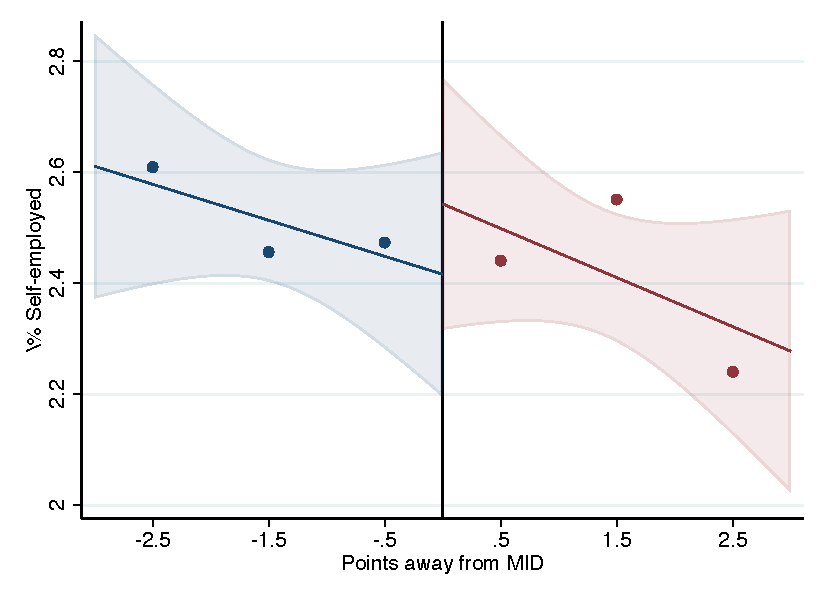
\includegraphics[width=\textwidth]{04_Figures/rd_plot_mid_age2018_pdelta3.pdf}
    \end{subfigure}

    \begin{subfigure}{0.475\textwidth}
        \centering
        \includegraphics[width=\textwidth]{04_Figures/rd_plot_tau_hombre_pdelta3.pdf}
    \end{subfigure}
    \begin{subfigure}{0.475\textwidth}
        \centering
        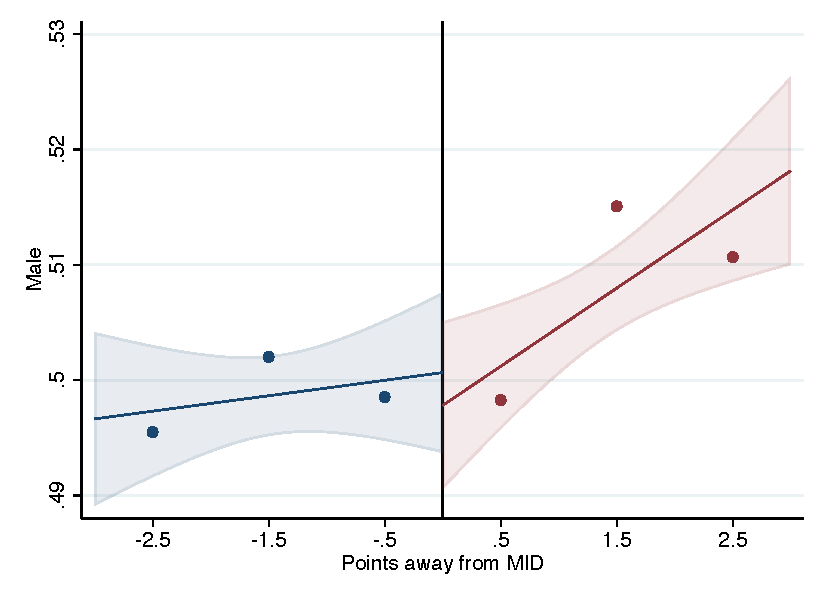
\includegraphics[width=\textwidth]{04_Figures/rd_plot_mid_hombre_pdelta3.pdf}
    \end{subfigure}

    \begin{subfigure}{0.475\textwidth}
        \centering
        \includegraphics[width=\textwidth]{04_Figures/rd_plot_tau_Secundaria_Privada_pdelta3.pdf}
    \end{subfigure}
    \begin{subfigure}{0.475\textwidth}
        \centering
        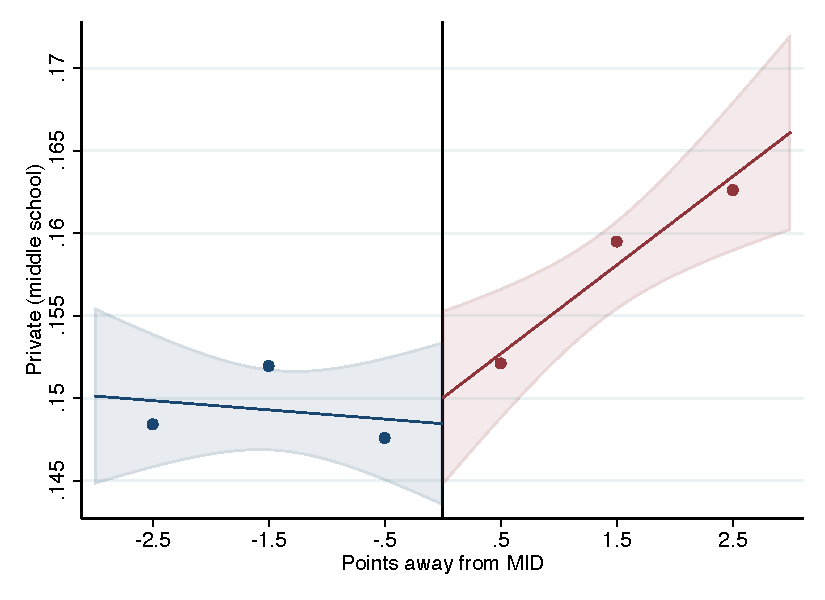
\includegraphics[width=\textwidth]{04_Figures/rd_plot_mid_Secundaria_Privada_pdelta3.pdf}
    \end{subfigure}
    \end{center}
    
\footnotesize
\textit{Notes}: Left side figures plot the regression discontinuity 3 points around the cutoff. Observations in the left side of the cutoff are ineligible to be assigned (controls), observations in the right side are eligible to be assigned (treated). Right side figures plot the regression discontinuity 3 points around the most informative disqualification (MID). Observations in the left side of the MID are eligible to be assigned (treated), observations in the right side are also eligible to be assigned, but they are also eligible at a higher ranked school (controls). All plots include students with marginal probability of being assigned to an elite school by the assignment mechanisms following \citet{abdulkadirouglu2022breaking}. 
\end{figure}

\begin{figure}[H]

    \ContinuedFloat
    \caption{(Continued) RD plots for balance variables across those assigned to either UNAM or IPN high-school, and those who are not\label{fig:Balance_rd_plot_elite_2}}
    \begin{center}
    
    \begin{subfigure}{0.475\textwidth}
        \centering
        \includegraphics[width=\textwidth]{04_Figures/rd_plot_tau_sus_prom_pdelta3.pdf}
    \end{subfigure}
    \begin{subfigure}{0.475\textwidth}
        \centering
        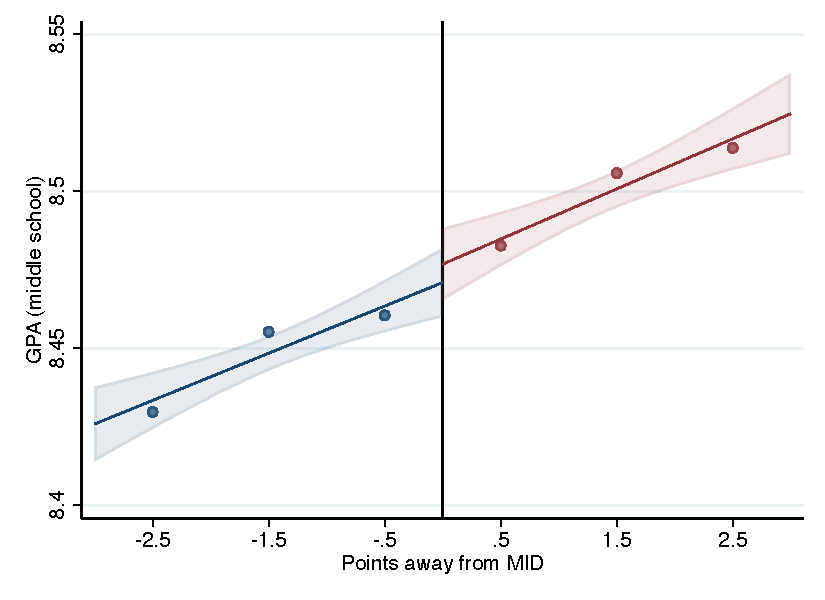
\includegraphics[width=\textwidth]{04_Figures/rd_plot_mid_sus_prom_pdelta3.pdf}
    \end{subfigure}

    \begin{subfigure}{0.475\textwidth}
        \centering
        \includegraphics[width=\textwidth]{04_Figures/rd_plot_tau_ano_cert_pdelta3.pdf}
    \end{subfigure}
    \begin{subfigure}{0.475\textwidth}
        \centering
        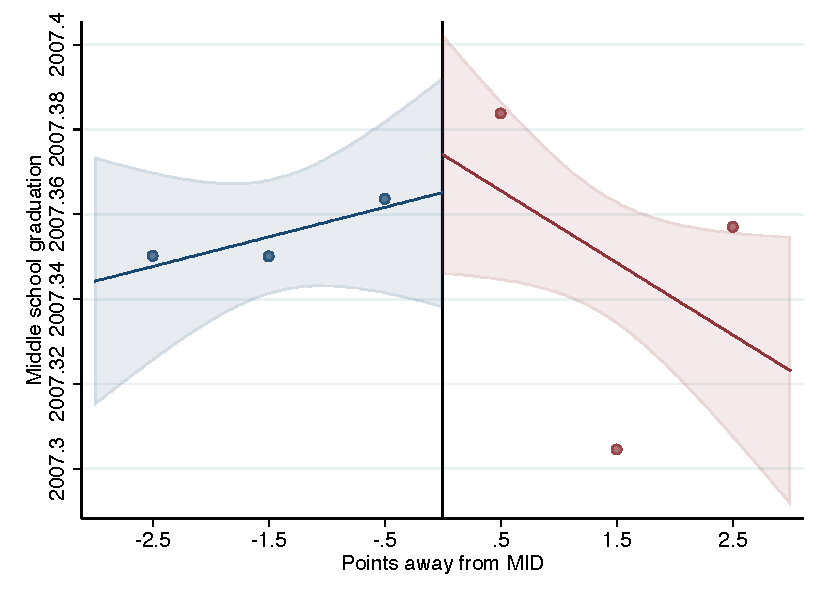
\includegraphics[width=\textwidth]{04_Figures/rd_plot_mid_ano_cert_pdelta3.pdf}
    \end{subfigure}

    \begin{subfigure}{0.475\textwidth}
        \centering
        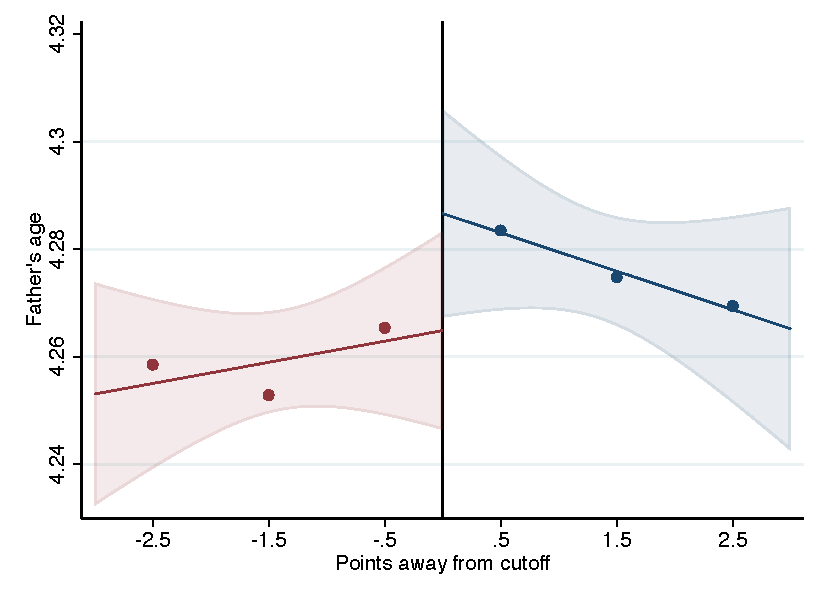
\includegraphics[width=\textwidth]{04_Figures/rd_plot_tau_edad_pad_pdelta3.pdf}
    \end{subfigure}
    \begin{subfigure}{0.475\textwidth}
        \centering
        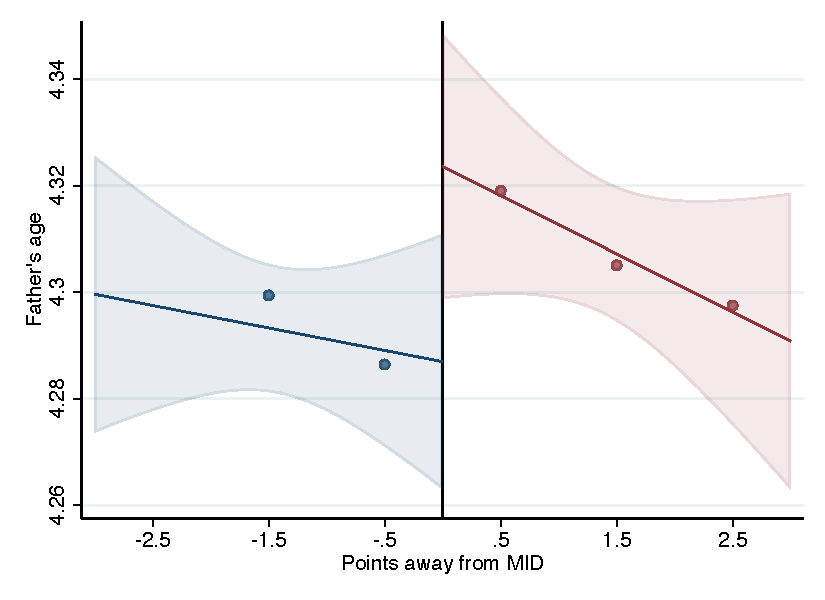
\includegraphics[width=\textwidth]{04_Figures/rd_plot_mid_edad_pad_pdelta3.pdf}
    \end{subfigure}
    \end{center}
    
\footnotesize
\textit{Notes}: Left side figures plot the regression discontinuity 3 points around the cutoff. Observations in the left side of the cutoff are ineligible to be assigned (controls), observations in the right side are eligible to be assigned (treated). Right side figures plot the regression discontinuity 3 points around the most informative disqualification (MID). Observations in the left side of the MID are eligible to be assigned (treated), observations in the right side are also eligible to be assigned, but they are also eligible at a higher ranked school (controls). All plots include students with marginal probability of being assigned to an elite school by the assignment mechanisms following \citet{abdulkadirouglu2022breaking}. 
\end{figure}

\begin{figure}[H]

    \ContinuedFloat
    \caption{(Continued) RD plots for balance variables across those assigned to either UNAM or IPN high-school, and those who are not\label{fig:Balance_rd_plot_elite_3}}
    \begin{center}

    \begin{subfigure}{0.475\textwidth}
        \centering
        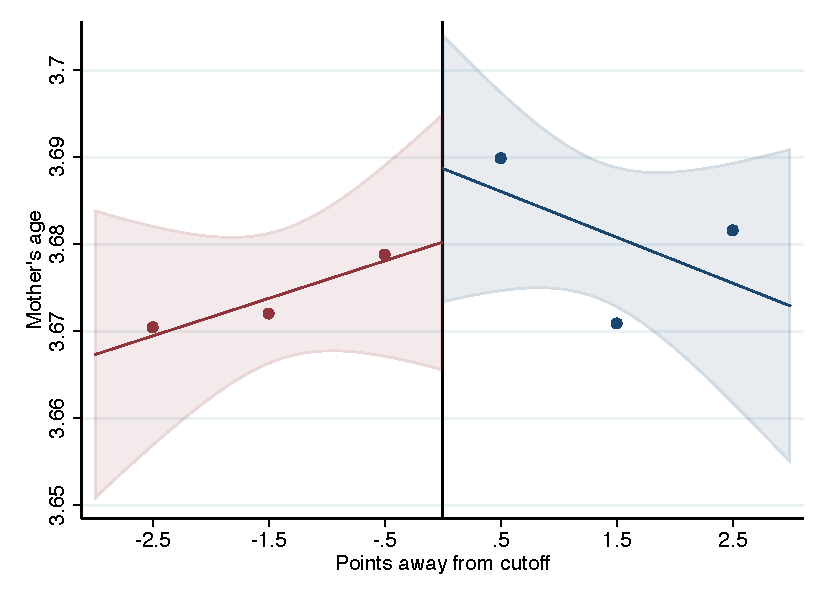
\includegraphics[width=\textwidth]{04_Figures/rd_plot_tau_edad_mad_pdelta3.pdf}
    \end{subfigure}
    \begin{subfigure}{0.475\textwidth}
        \centering
        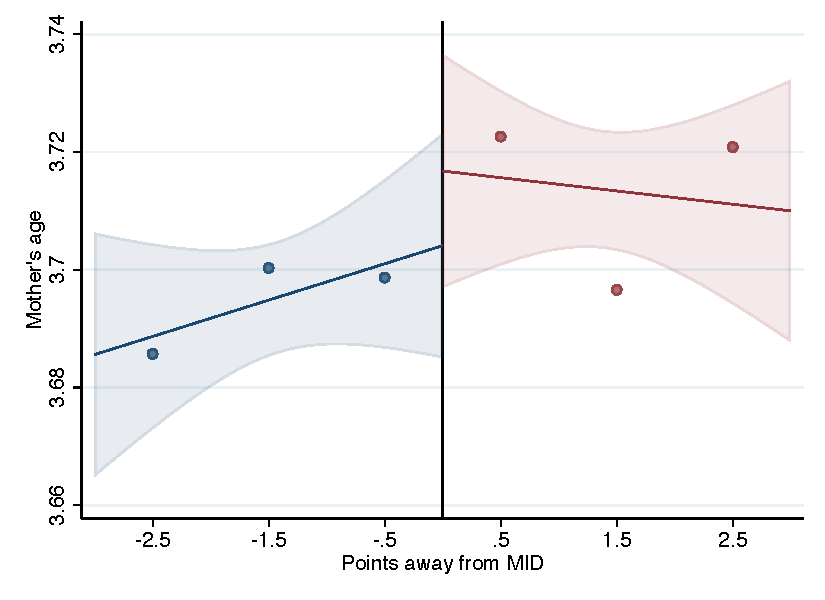
\includegraphics[width=\textwidth]{04_Figures/rd_plot_mid_edad_mad_pdelta3.pdf}
    \end{subfigure}
    \end{center}
    
\footnotesize
\textit{Notes}: Left side figures plot the regression discontinuity 3 points around the cutoff. Observations in the left side of the cutoff are ineligible to be assigned (controls), observations in the right side are eligible to be assigned (treated). Right side figures plot the regression discontinuity 3 points around the most informative disqualification (MID). Observations in the left side of the MID are eligible to be assigned (treated), observations in the right side are also eligible to be assigned, but they are also eligible at a higher ranked school (controls). All plots include students with marginal probability of being assigned to an elite school by the assignment mechanisms following \citet{abdulkadirouglu2022breaking}. 
\end{figure}

\subsubsection{IPN assignments}

\begin{figure}[H]

    \caption{RD plots for balance variables across those assigned to IPN high-school, and those who are not\label{fig:Balance_rd_plot_IPN_1}}
    \begin{center}
    
    \begin{subfigure}{0.475\textwidth}
        \centering
        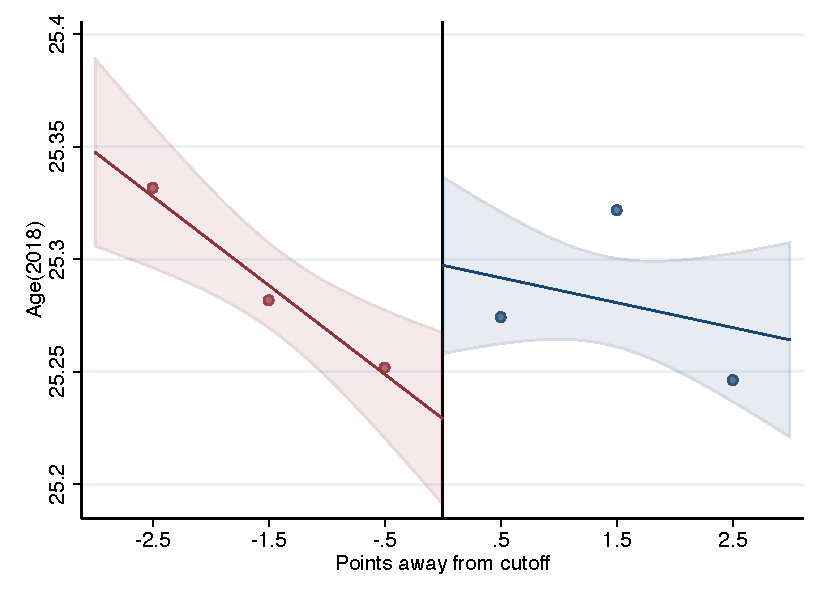
\includegraphics[width=\textwidth]{04_Figures/rd_plot_tau_age2018_IPN3.pdf}
    \end{subfigure}
    \begin{subfigure}{0.475\textwidth}
        \centering
        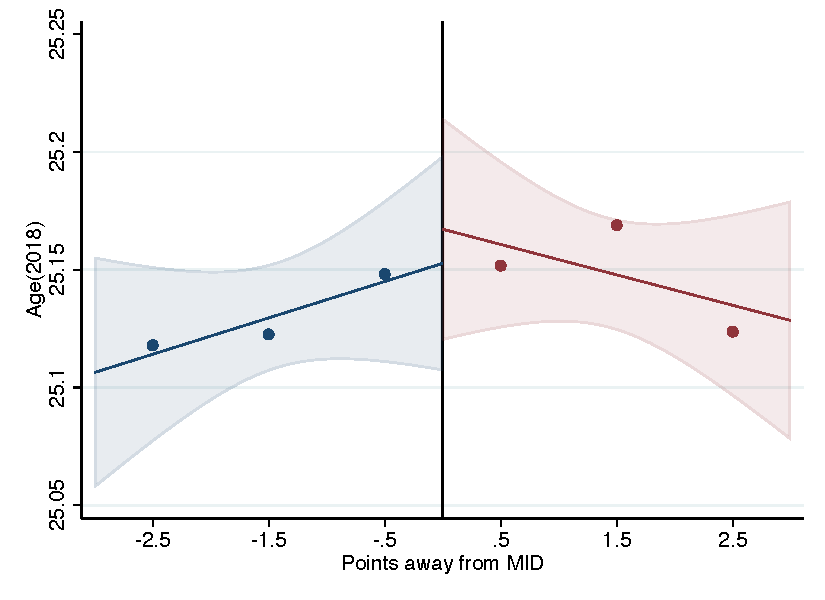
\includegraphics[width=\textwidth]{04_Figures/rd_plot_mid_age2018_IPN3.pdf}
    \end{subfigure}

    \begin{subfigure}{0.475\textwidth}
        \centering
        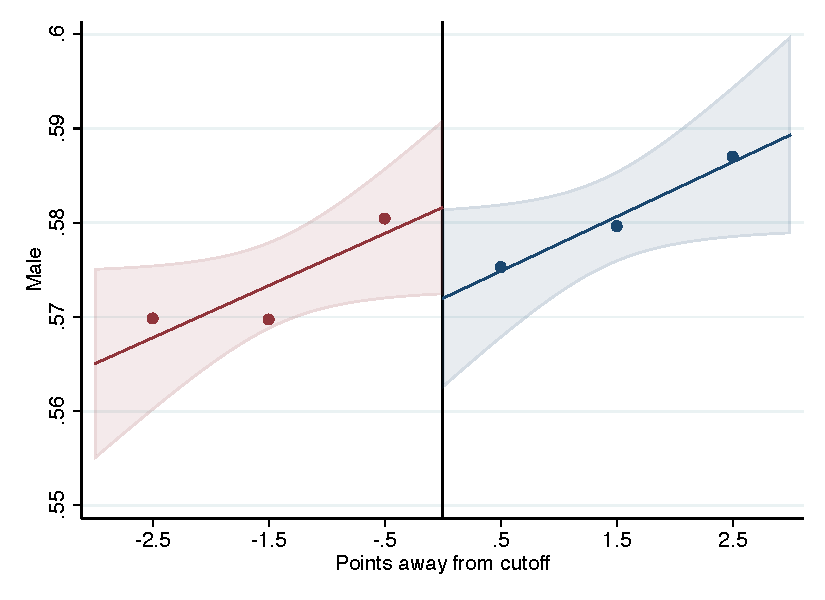
\includegraphics[width=\textwidth]{04_Figures/rd_plot_tau_hombre_IPN3.pdf}
    \end{subfigure}
    \begin{subfigure}{0.475\textwidth}
        \centering
        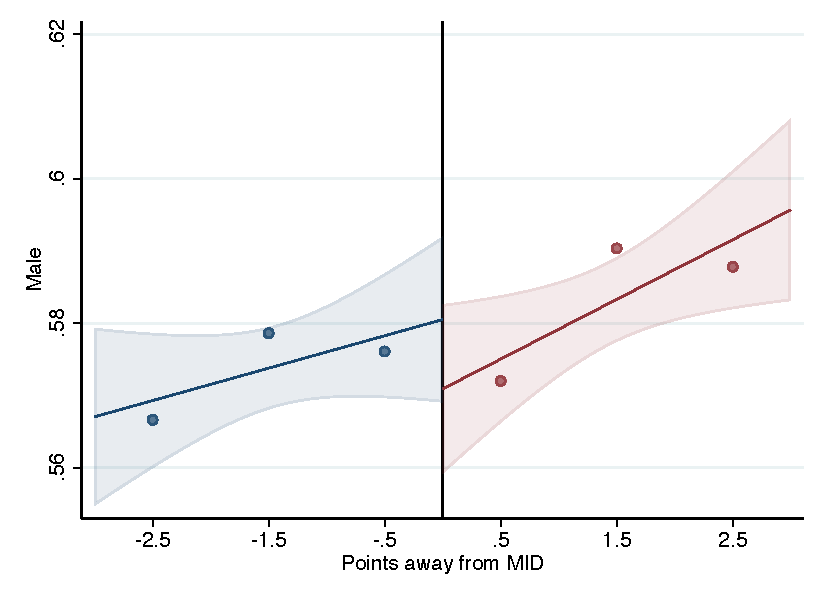
\includegraphics[width=\textwidth]{04_Figures/rd_plot_mid_hombre_IPN3.pdf}
    \end{subfigure}

    \begin{subfigure}{0.475\textwidth}
        \centering
        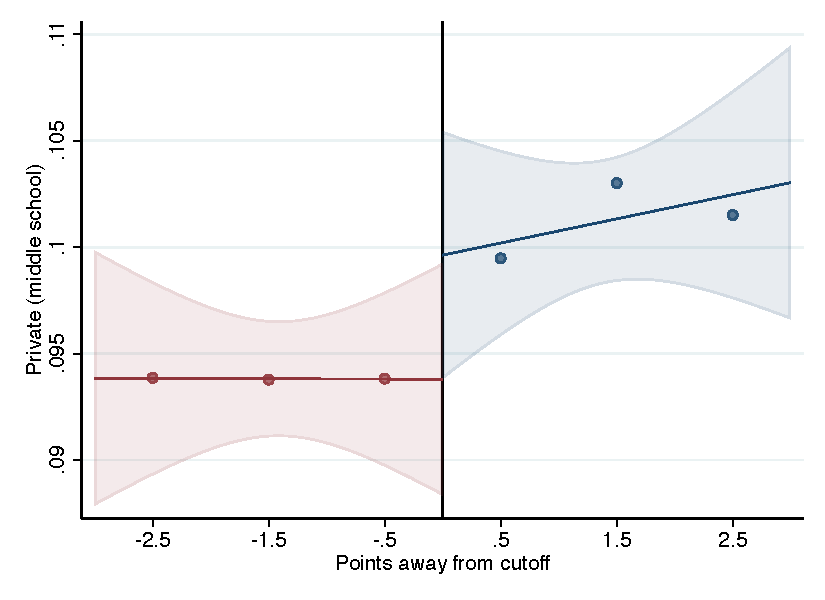
\includegraphics[width=\textwidth]{04_Figures/rd_plot_tau_Secundaria_Privada_IPN3.pdf}
    \end{subfigure}
    \begin{subfigure}{0.475\textwidth}
        \centering
        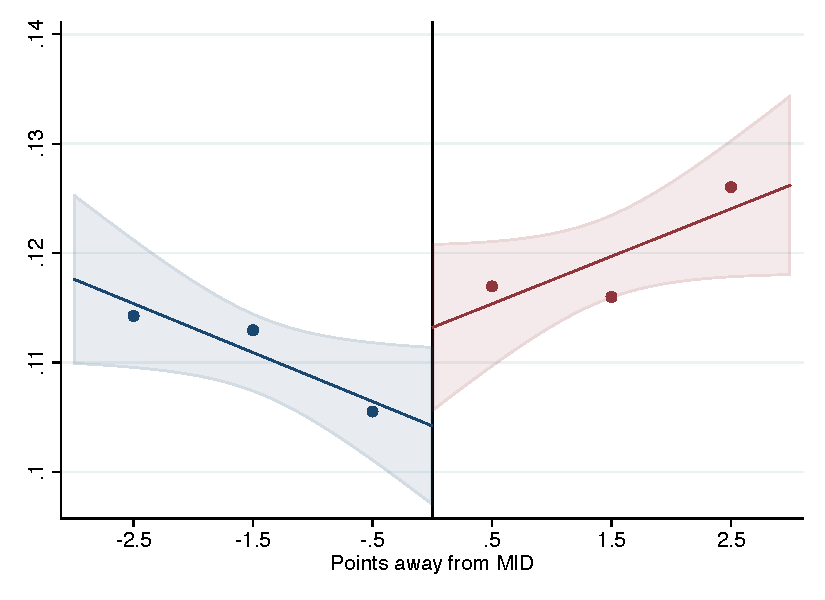
\includegraphics[width=\textwidth]{04_Figures/rd_plot_mid_Secundaria_Privada_IPN3.pdf}
    \end{subfigure}
    \end{center}
    
\footnotesize
\textit{Notes}: Left side figures plot the regression discontinuity 3 points around the cutoff. Observations in the left side of the cutoff are ineligible to be assigned (controls), observations in the right side are eligible to be assigned (treated). Right side figures plot the regression discontinuity 3 points around the most informative disqualification (MID). Observations in the left side of the MID are eligible to be assigned (treated), observations in the right side are also eligible to be assigned, but they are also eligible at a higher ranked school (controls). All plots include students with marginal probability of being assigned to an elite school by the assignment mechanisms following \citet{abdulkadirouglu2022breaking}. 
\end{figure}

\begin{figure}[H]

    \ContinuedFloat
    \caption{(Continued) RD plots for balance variables across those assigned to IPN high-school, and those who are not\label{fig:Balance_rd_plot_IPN_2}}
    \begin{center}
    
    \begin{subfigure}{0.475\textwidth}
        \centering
        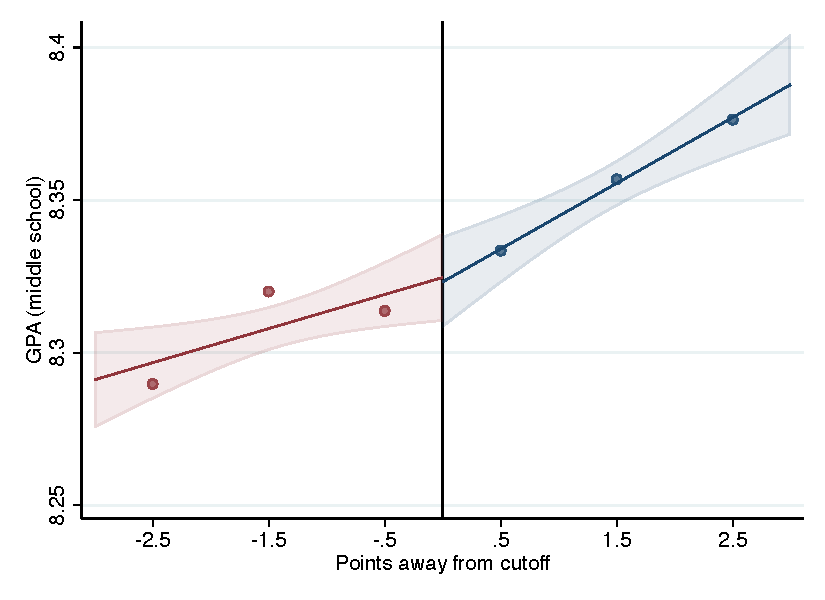
\includegraphics[width=\textwidth]{04_Figures/rd_plot_tau_sus_prom_IPN3.pdf}
    \end{subfigure}
    \begin{subfigure}{0.475\textwidth}
        \centering
        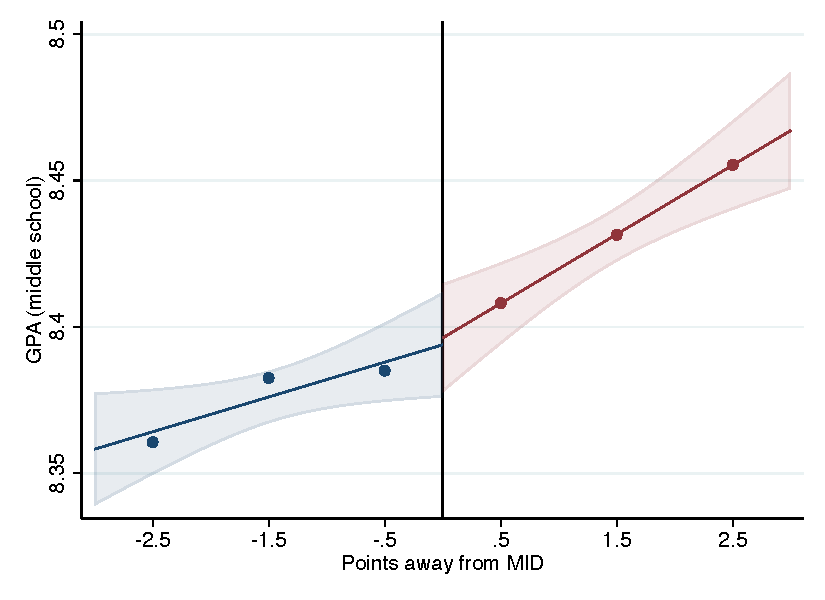
\includegraphics[width=\textwidth]{04_Figures/rd_plot_mid_sus_prom_IPN3.pdf}
    \end{subfigure}

    \begin{subfigure}{0.475\textwidth}
        \centering
        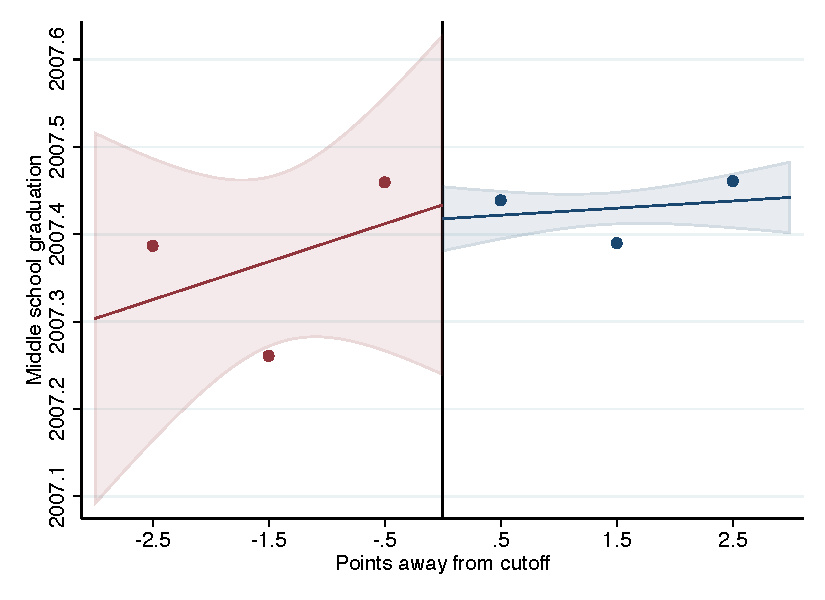
\includegraphics[width=\textwidth]{04_Figures/rd_plot_tau_ano_cert_IPN3.pdf}
    \end{subfigure}
    \begin{subfigure}{0.475\textwidth}
        \centering
        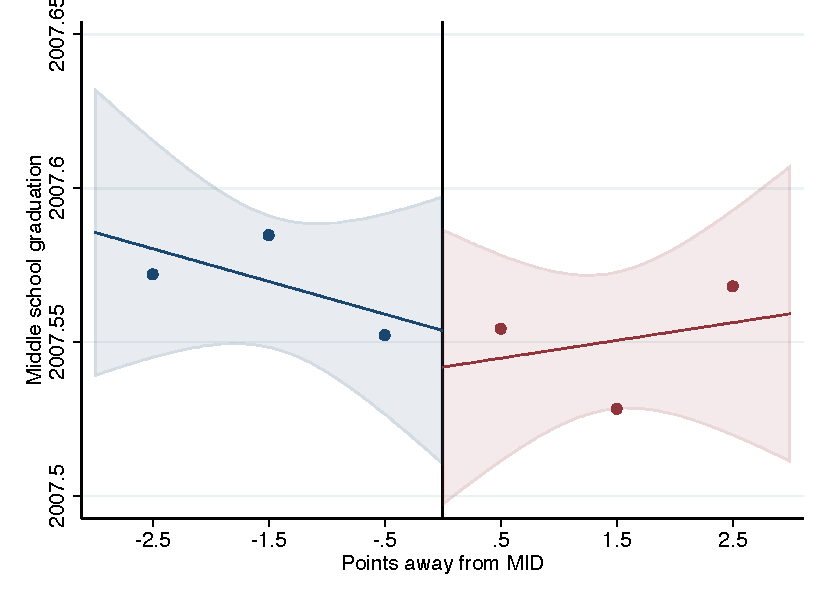
\includegraphics[width=\textwidth]{04_Figures/rd_plot_mid_ano_cert_IPN3.pdf}
    \end{subfigure}

    \begin{subfigure}{0.475\textwidth}
        \centering
        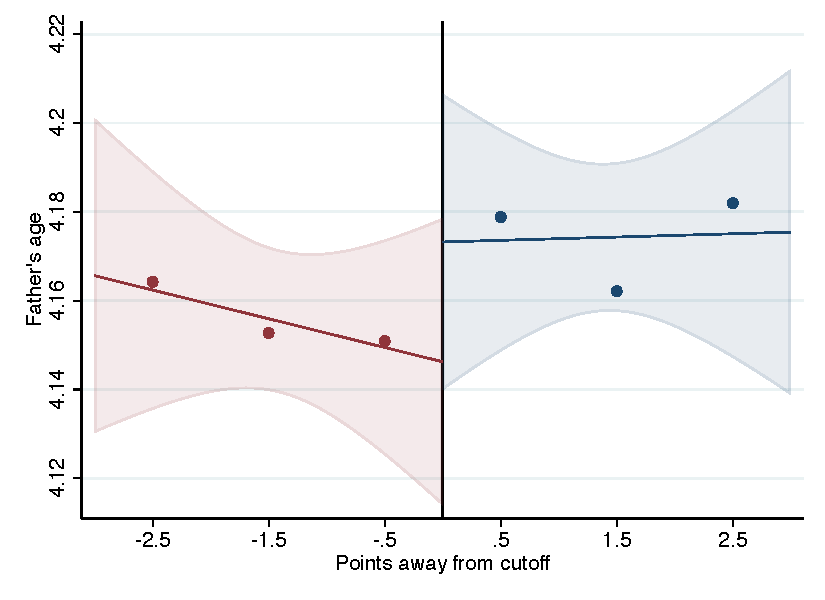
\includegraphics[width=\textwidth]{04_Figures/rd_plot_tau_edad_pad_IPN3.pdf}
    \end{subfigure}
    \begin{subfigure}{0.475\textwidth}
        \centering
        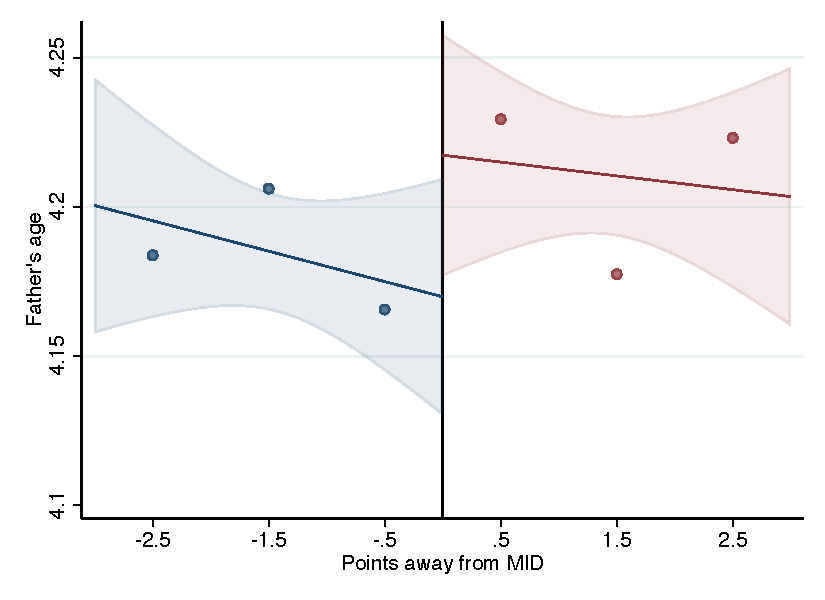
\includegraphics[width=\textwidth]{04_Figures/rd_plot_mid_edad_pad_IPN3.pdf}
    \end{subfigure}
    \end{center}
    
\footnotesize
\textit{Notes}: Left side figures plot the regression discontinuity 3 points around the cutoff. Observations in the left side of the cutoff are ineligible to be assigned (controls), observations in the right side are eligible to be assigned (treated). Right side figures plot the regression discontinuity 3 points around the most informative disqualification (MID). Observations in the left side of the MID are eligible to be assigned (treated), observations in the right side are also eligible to be assigned, but they are also eligible at a higher ranked school (controls). All plots include students with marginal probability of being assigned to an elite school by the assignment mechanisms following \citet{abdulkadirouglu2022breaking}. 
\end{figure}

\begin{figure}[H]

    \ContinuedFloat
    \caption{(Continued) RD plots for balance variables across those assigned to IPN high-school, and those who are not\label{fig:Balance_rd_plot_IPN_3}}
    \begin{center}

    \begin{subfigure}{0.475\textwidth}
        \centering
        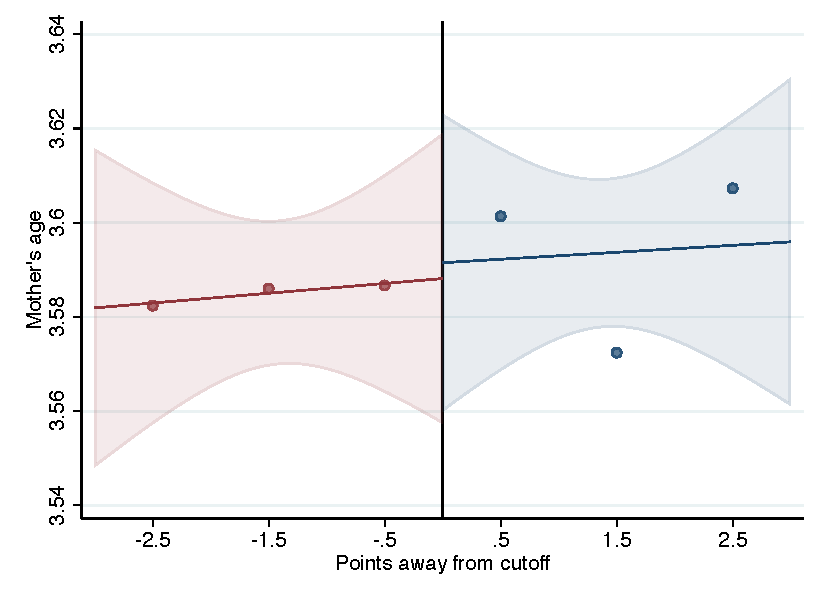
\includegraphics[width=\textwidth]{04_Figures/rd_plot_tau_edad_mad_IPN3.pdf}
    \end{subfigure}
    \begin{subfigure}{0.475\textwidth}
        \centering
        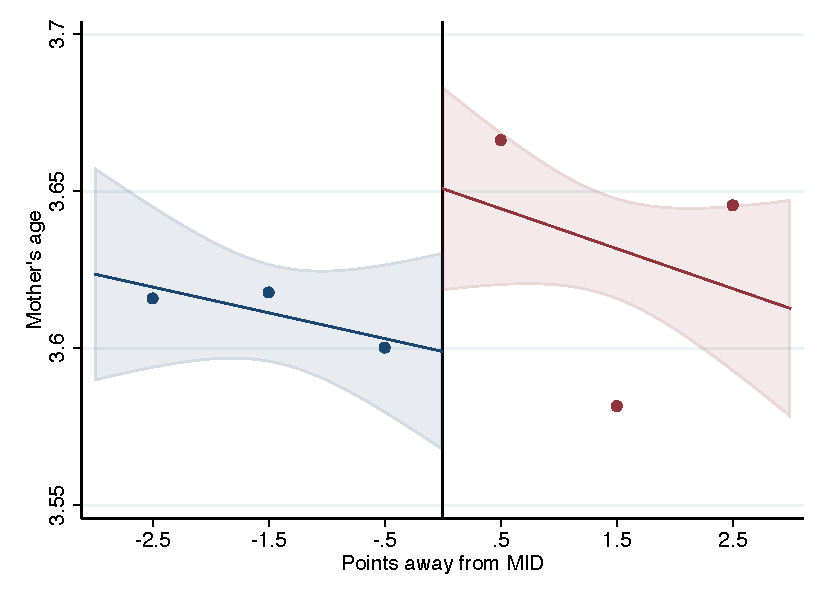
\includegraphics[width=\textwidth]{04_Figures/rd_plot_mid_edad_mad_IPN3.pdf}
    \end{subfigure}
    \end{center}
    
\footnotesize
\textit{Notes}: Left side figures plot the regression discontinuity 3 points around the cutoff. Observations in the left side of the cutoff are ineligible to be assigned (controls), observations in the right side are eligible to be assigned (treated). Right side figures plot the regression discontinuity 3 points around the most informative disqualification (MID). Observations in the left side of the MID are eligible to be assigned (treated), observations in the right side are also eligible to be assigned, but they are also eligible at a higher ranked school (controls). All plots include students with marginal probability of being assigned to an elite school by the assignment mechanisms following \citet{abdulkadirouglu2022breaking}. 
\end{figure}

\subsubsection{UNAM assignments}

\begin{figure}[H]

    \caption{RD plots for balance variables across those assigned to UNAM high-school, and those who are not\label{fig:Balance_rd_plot_UNAM_1}}
    \begin{center}
    
    \begin{subfigure}{0.475\textwidth}
        \centering
        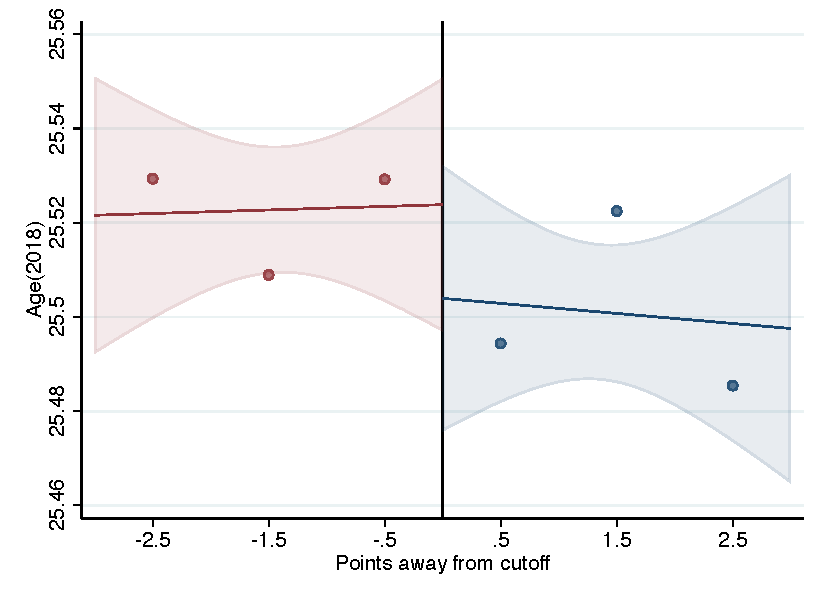
\includegraphics[width=\textwidth]{04_Figures/rd_plot_tau_age2018_UNAM3.pdf}
    \end{subfigure}
    \begin{subfigure}{0.475\textwidth}
        \centering
        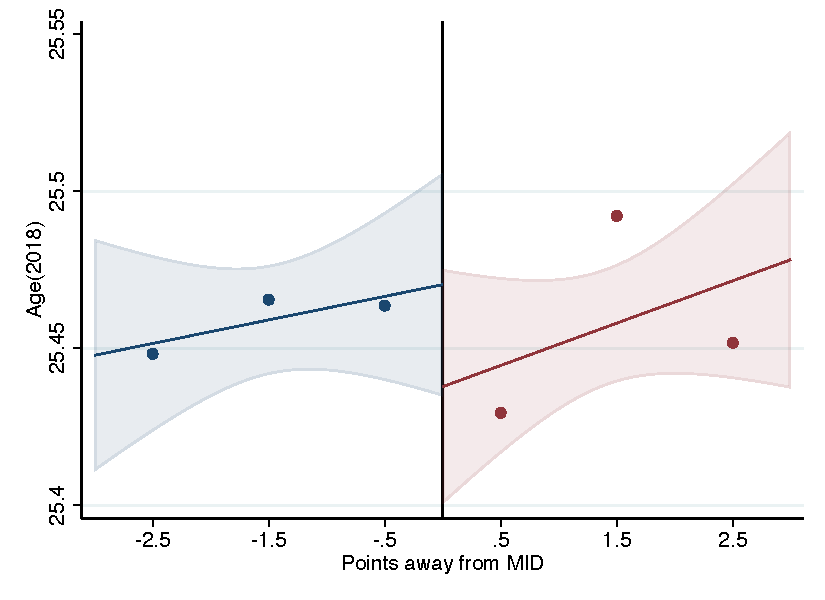
\includegraphics[width=\textwidth]{04_Figures/rd_plot_mid_age2018_UNAM3.pdf}
    \end{subfigure}

    \begin{subfigure}{0.475\textwidth}
        \centering
        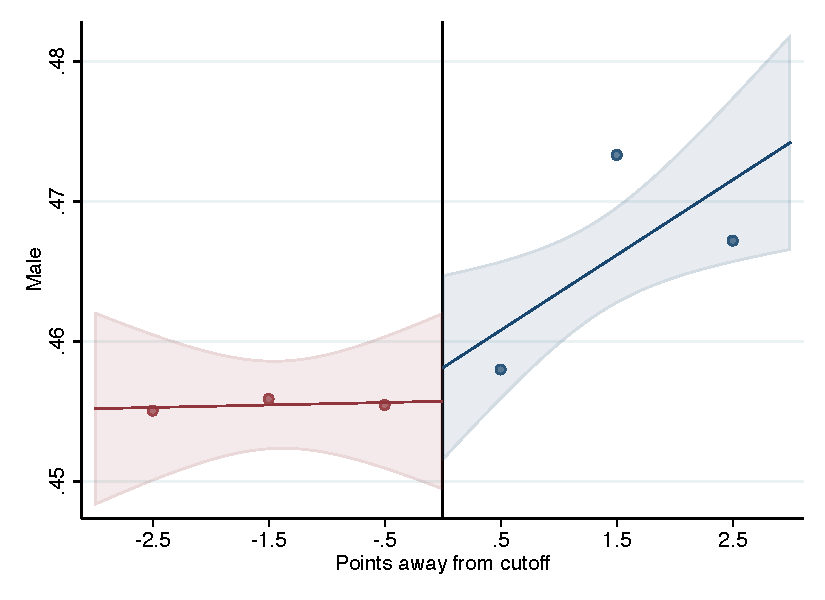
\includegraphics[width=\textwidth]{04_Figures/rd_plot_tau_hombre_UNAM3.pdf}
    \end{subfigure}
    \begin{subfigure}{0.475\textwidth}
        \centering
        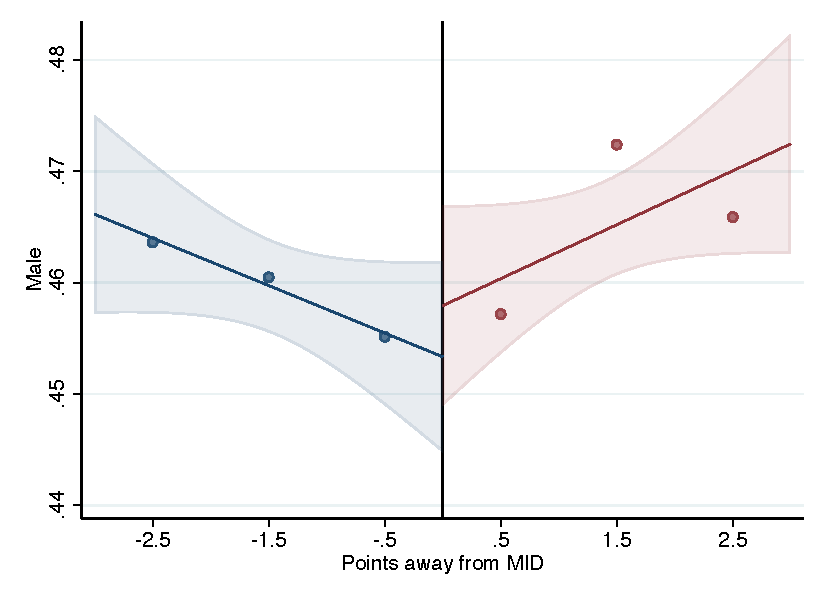
\includegraphics[width=\textwidth]{04_Figures/rd_plot_mid_hombre_UNAM3.pdf}
    \end{subfigure}

    \begin{subfigure}{0.475\textwidth}
        \centering
        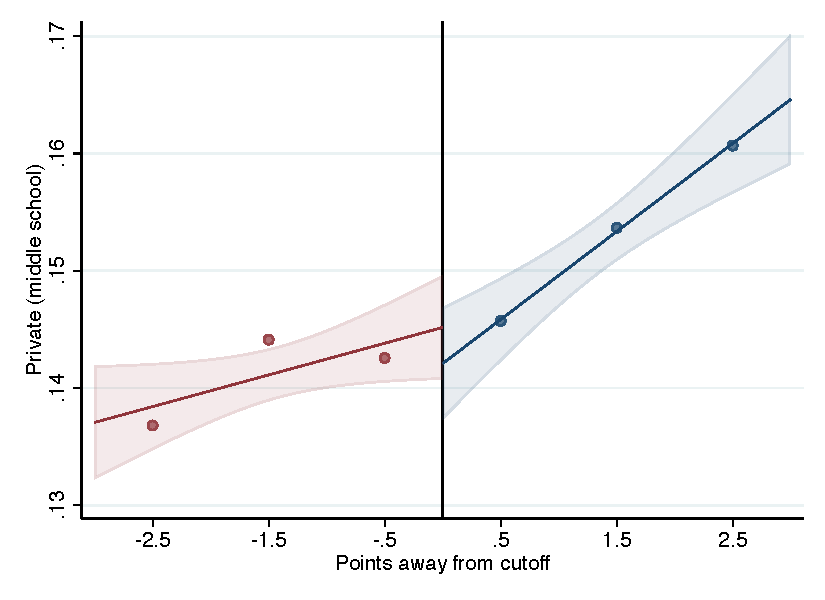
\includegraphics[width=\textwidth]{04_Figures/rd_plot_tau_Secundaria_Privada_UNAM3.pdf}
    \end{subfigure}
    \begin{subfigure}{0.475\textwidth}
        \centering
        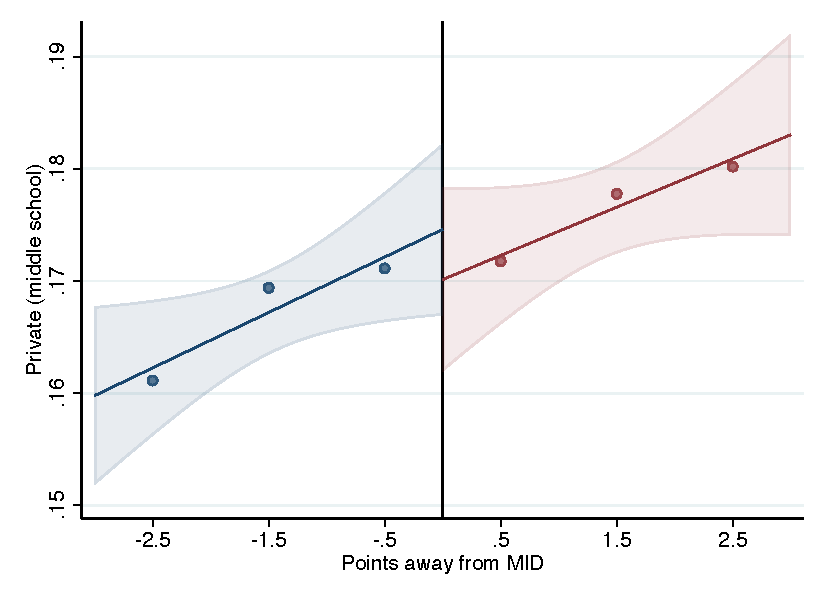
\includegraphics[width=\textwidth]{04_Figures/rd_plot_mid_Secundaria_Privada_UNAM3.pdf}
    \end{subfigure}
    \end{center}
    
\footnotesize
\textit{Notes}: Left side figures plot the regression discontinuity 3 points around the cutoff. Observations in the left side of the cutoff are ineligible to be assigned (controls), observations in the right side are eligible to be assigned (treated). Right side figures plot the regression discontinuity 3 points around the most informative disqualification (MID). Observations in the left side of the MID are eligible to be assigned (treated), observations in the right side are also eligible to be assigned, but they are also eligible at a higher ranked school (controls). All plots include students with marginal probability of being assigned to an elite school by the assignment mechanisms following \citet{abdulkadirouglu2022breaking}. 
\end{figure}

\begin{figure}[H]

    \ContinuedFloat
    \caption{(Continued) RD plots for balance variables across those assigned to UNAM high-school, and those who are not\label{fig:Balance_rd_plot_UNAM_2}}
    \begin{center}
    
    \begin{subfigure}{0.475\textwidth}
        \centering
        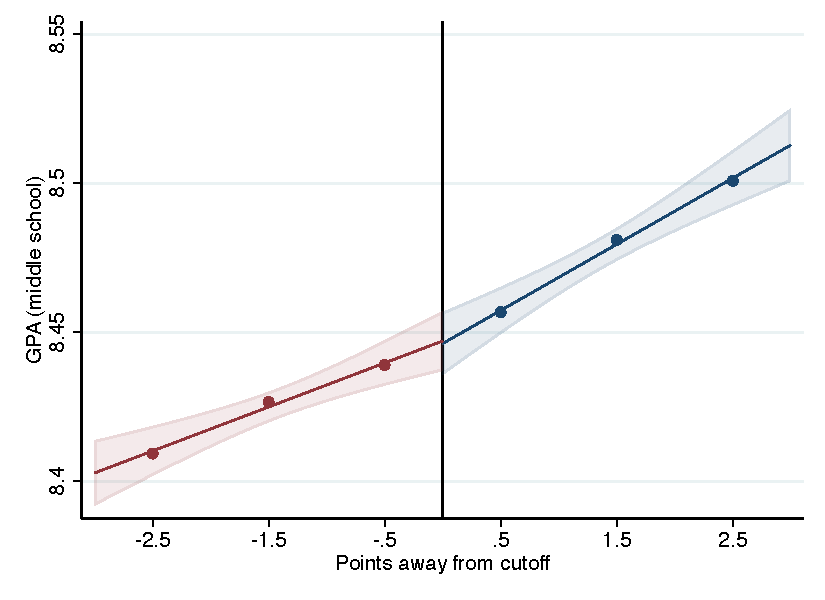
\includegraphics[width=\textwidth]{04_Figures/rd_plot_tau_sus_prom_UNAM3.pdf}
    \end{subfigure}
    \begin{subfigure}{0.475\textwidth}
        \centering
        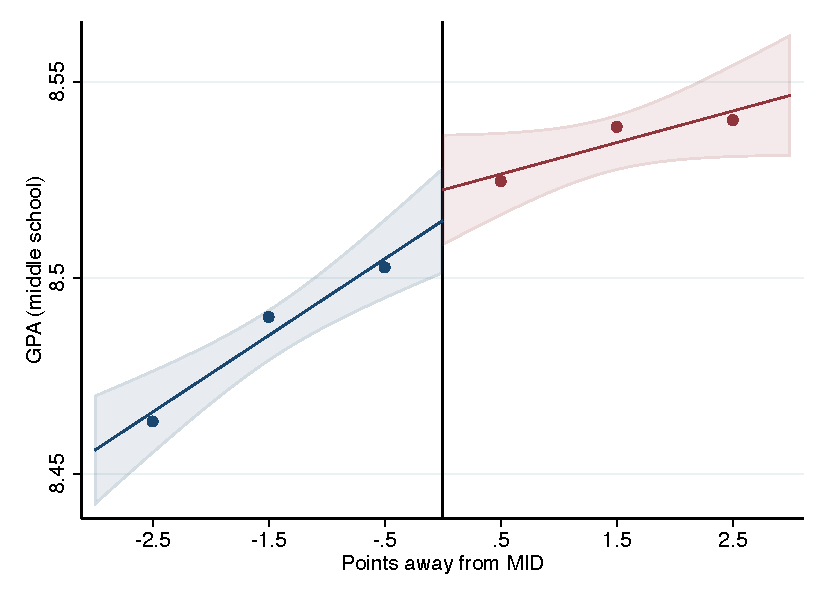
\includegraphics[width=\textwidth]{04_Figures/rd_plot_mid_sus_prom_UNAM3.pdf}
    \end{subfigure}

    \begin{subfigure}{0.475\textwidth}
        \centering
        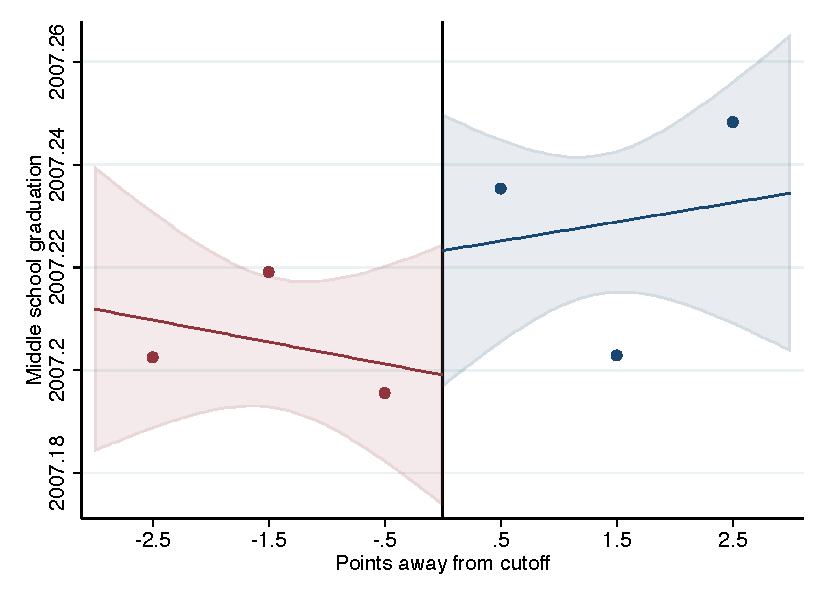
\includegraphics[width=\textwidth]{04_Figures/rd_plot_tau_ano_cert_UNAM3.pdf}
    \end{subfigure}
    \begin{subfigure}{0.475\textwidth}
        \centering
        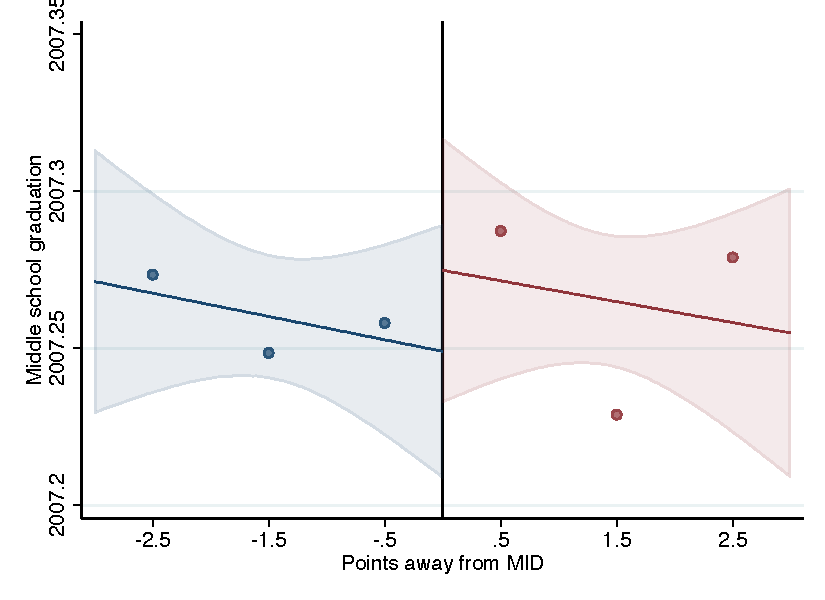
\includegraphics[width=\textwidth]{04_Figures/rd_plot_mid_ano_cert_UNAM3.pdf}
    \end{subfigure}

    \begin{subfigure}{0.475\textwidth}
        \centering
        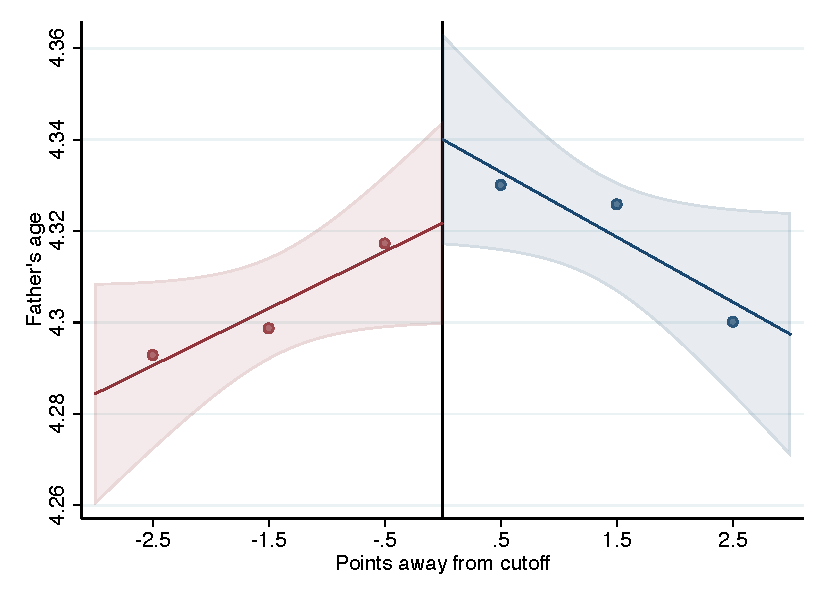
\includegraphics[width=\textwidth]{04_Figures/rd_plot_tau_edad_pad_UNAM3.pdf}
    \end{subfigure}
    \begin{subfigure}{0.475\textwidth}
        \centering
        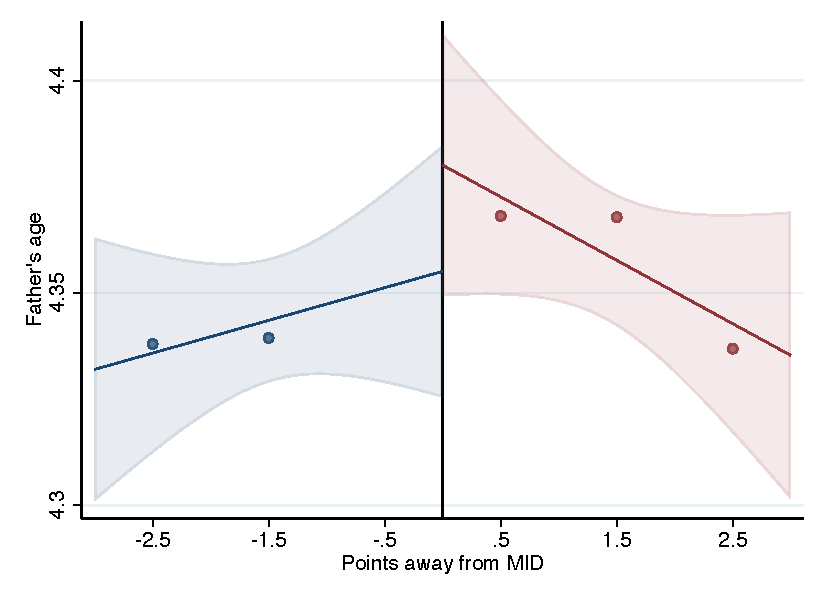
\includegraphics[width=\textwidth]{04_Figures/rd_plot_mid_edad_pad_UNAM3.pdf}
    \end{subfigure}
    \end{center}
    
\footnotesize
\textit{Notes}: Left side figures plot the regression discontinuity 3 points around the cutoff. Observations in the left side of the cutoff are ineligible to be assigned (controls), observations in the right side are eligible to be assigned (treated). Right side figures plot the regression discontinuity 3 points around the most informative disqualification (MID). Observations in the left side of the MID are eligible to be assigned (treated), observations in the right side are also eligible to be assigned, but they are also eligible at a higher ranked school (controls). All plots include students with marginal probability of being assigned to an elite school by the assignment mechanisms following \citet{abdulkadirouglu2022breaking}. 
\end{figure}

\begin{figure}[H]

    \ContinuedFloat
    \caption{(Continued) RD plots for balance variables across those assigned to UNAM high-school, and those who are not\label{fig:Balance_rd_plot_UNAM_3}}
    \begin{center}

    \begin{subfigure}{0.475\textwidth}
        \centering
        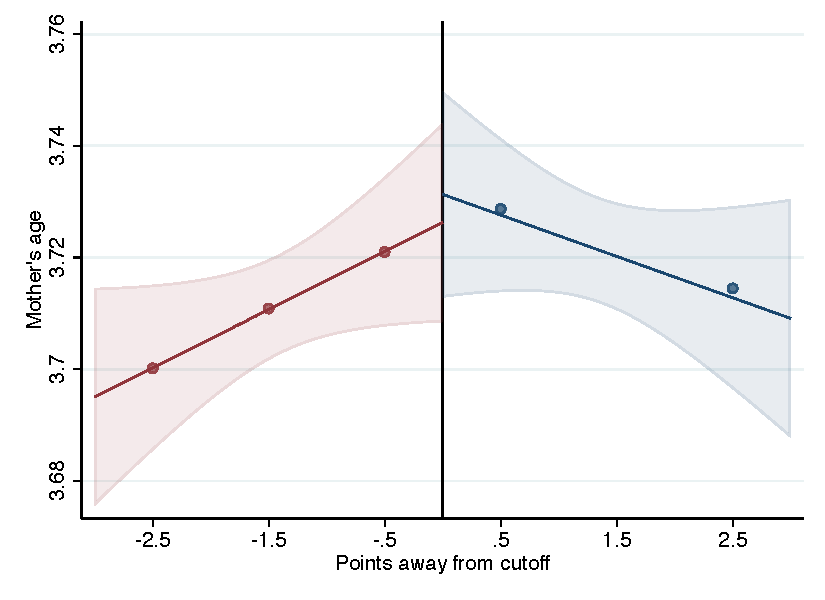
\includegraphics[width=\textwidth]{04_Figures/rd_plot_tau_edad_mad_UNAM3.pdf}
    \end{subfigure}
    \begin{subfigure}{0.475\textwidth}
        \centering
        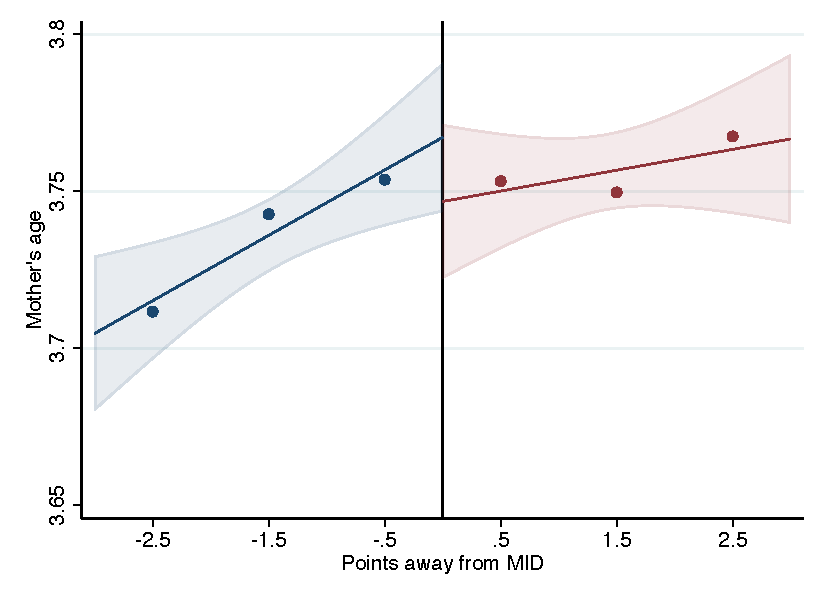
\includegraphics[width=\textwidth]{04_Figures/rd_plot_mid_edad_mad_UNAM3.pdf}
    \end{subfigure}
    \end{center}
    
\footnotesize
\textit{Notes}: Left side figures plot the regression discontinuity 3 points around the cutoff. Observations in the left side of the cutoff are ineligible to be assigned (controls), observations in the right side are eligible to be assigned (treated). Right side figures plot the regression discontinuity 3 points around the most informative disqualification (MID). Observations in the left side of the MID are eligible to be assigned (treated), observations in the right side are also eligible to be assigned, but they are also eligible at a higher ranked school (controls). All plots include students with marginal probability of being assigned to an elite school by the assignment mechanisms following \citet{abdulkadirouglu2022breaking}. 
\end{figure}

\subsection{Treatment RD plots}

\begin{figure}[H]

    \caption{RD plots for treatment variables\label{fig:treat_rd_plot}}
    \begin{center}
    
    \begin{subfigure}{0.475\textwidth}
        \caption{IPN or UNAM assignment around cutoff}
        \centering
        \includegraphics[width=\textwidth]{04_Figures/rd_plot_tau_Elite_assig_pdelta3.pdf}
    \end{subfigure}
    \begin{subfigure}{0.475\textwidth}
        \caption{IPN or UNAM assignment around MID}
        \centering
        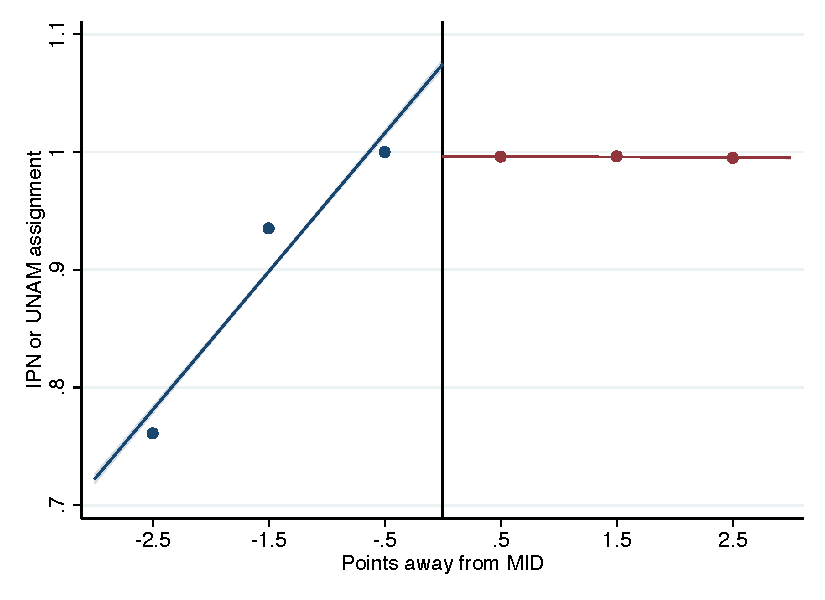
\includegraphics[width=\textwidth]{04_Figures/rd_plot_mid_Elite_assig_pdelta3.pdf}
    \end{subfigure}

    \begin{subfigure}{0.475\textwidth}
        \caption{IPN assignment around cutoff}
        \centering
        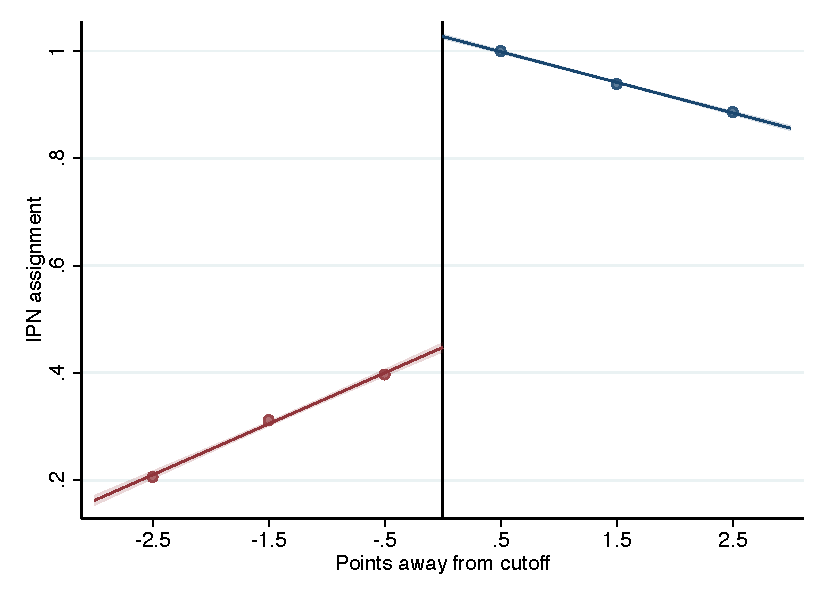
\includegraphics[width=\textwidth]{04_Figures/rd_plot_tau_IPN_assig_IPN3.pdf}
    \end{subfigure}
    \begin{subfigure}{0.475\textwidth}
        \caption{IPN assignment around MID}
        \centering
        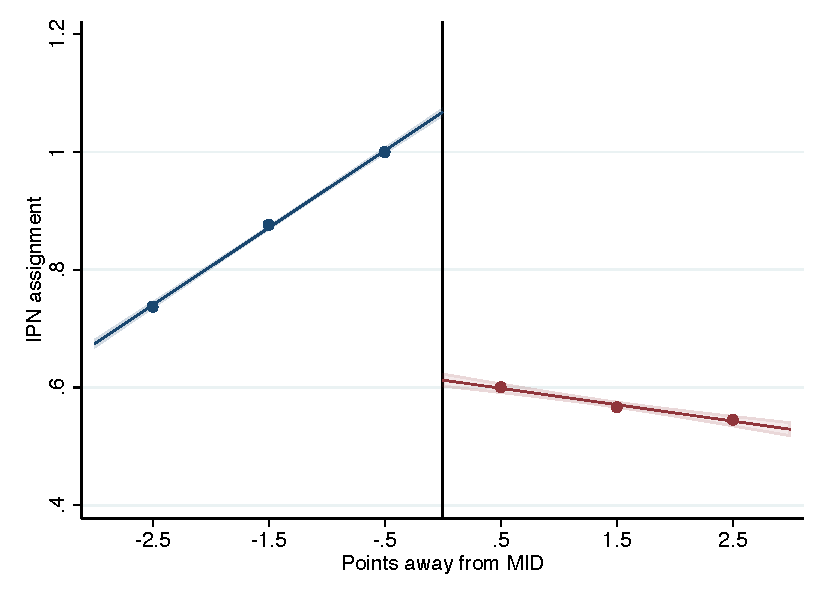
\includegraphics[width=\textwidth]{04_Figures/rd_plot_mid_IPN_assig_IPN3.pdf}
    \end{subfigure}

    \begin{subfigure}{0.475\textwidth}
        \caption{UNAM assignment around cutoff}
        \centering
        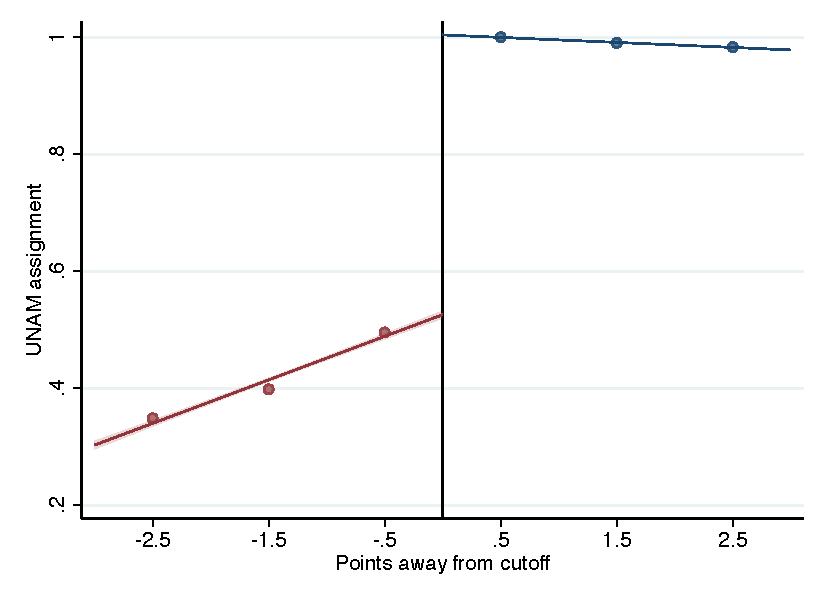
\includegraphics[width=\textwidth]{04_Figures/rd_plot_tau_UNAM_assig_UNAM3.pdf}
    \end{subfigure}
    \begin{subfigure}{0.475\textwidth}
        \caption{UNAM assignment around MID}
        \centering
        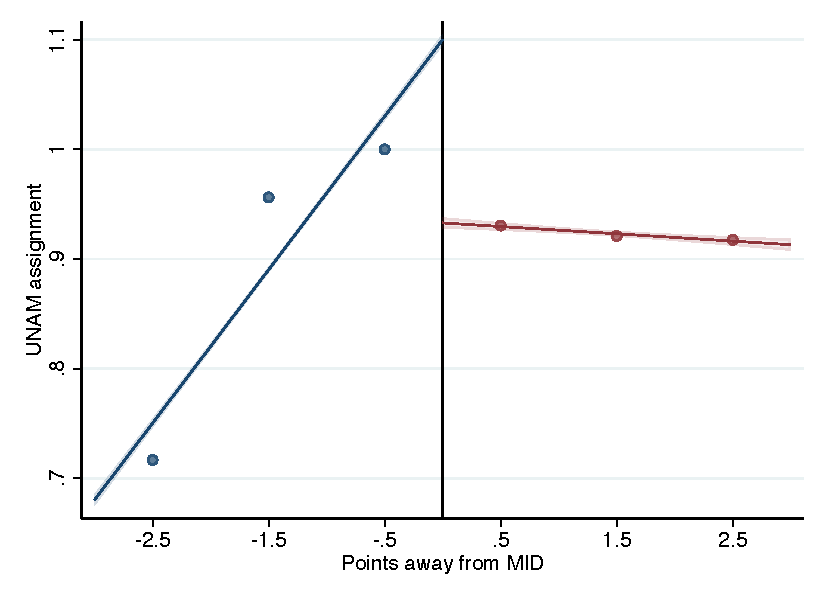
\includegraphics[width=\textwidth]{04_Figures/rd_plot_mid_UNAM_assig_UNAM3.pdf}
    \end{subfigure}
    \end{center}
    
\footnotesize
\textit{Notes}: Left side figures plot the regression discontinuity 3 points around the cutoff. Observations in the left side of the cutoff are ineligible to be assigned (controls), observations in the right side are eligible to be assigned (treated). Right side figures plot the regression discontinuity 3 points around the most informative disqualification (MID). Observations in the left side of the MID are eligible to be assigned (treated), observations in the right side are also eligible to be assigned, but they are also eligible at a higher ranked school (controls). All plots include students with marginal probability of being assigned to an elite school by the assignment mechanisms following \citet{abdulkadirouglu2022breaking}. 
\end{figure}

\subsection{Intent to treat RD plots}

\subsubsection{UNAM or IPN assignments}

\begin{figure}[H]

    \caption{RD plots for outcome variables across those assigned to either UNAM or IPN high-school, and those who are not\label{fig:ITT_rd_plot_elite_1}}
    \begin{center}
    
    \begin{subfigure}{0.475\textwidth}
        \centering
        \includegraphics[width=\textwidth]{04_Figures/rd_plot_tau_ENLACE_ANY_pdelta3.pdf}
    \end{subfigure}
    \begin{subfigure}{0.475\textwidth}
        \centering
        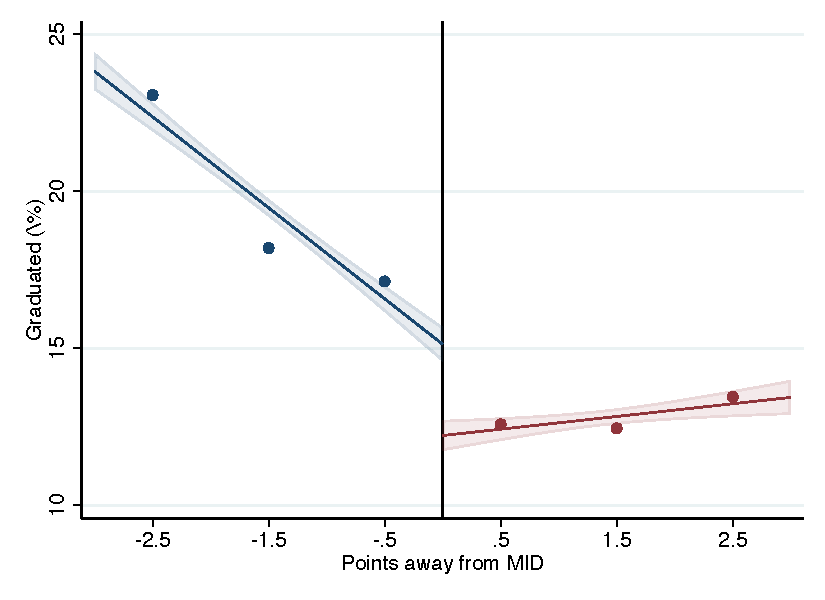
\includegraphics[width=\textwidth]{04_Figures/rd_plot_mid_ENLACE_ANY_pdelta3.pdf}
    \end{subfigure}

    \begin{subfigure}{0.475\textwidth}
        \centering
        \includegraphics[width=\textwidth]{04_Figures/rd_plot_tau_ENLACE_Privado_Un_pdelta3.pdf}
    \end{subfigure}
    \begin{subfigure}{0.475\textwidth}
        \centering
        \includegraphics[width=\textwidth]{04_Figures/rd_plot_mid_ENLACE_Privado_Un_pdelta3.pdf}
    \end{subfigure}

    \begin{subfigure}{0.475\textwidth}
        \centering
        \includegraphics[width=\textwidth]{04_Figures/rd_plot_tau_ENLACE_Privado_pdelta3.pdf}
    \end{subfigure}
    \begin{subfigure}{0.475\textwidth}
        \centering
        \includegraphics[width=\textwidth]{04_Figures/rd_plot_mid_ENLACE_Privado_pdelta3.pdf}
    \end{subfigure}
    \end{center}
    
\footnotesize
\textit{Notes}: Left side figures plot the regression discontinuity 3 points around the cutoff. Observations in the left side of the cutoff are ineligible to be assigned (controls), observations in the right side are eligible to be assigned (treated). Right side figures plot the regression discontinuity 3 points around the most informative disqualification (MID). Observations in the left side of the MID are eligible to be assigned (treated), observations in the right side are also eligible to be assigned, but they are also eligible at a higher ranked school (controls). All plots include students with marginal probability of being assigned to an elite school by the assignment mechanisms following \citet{abdulkadirouglu2022breaking}. 
\end{figure}

\begin{figure}[H]

    \ContinuedFloat
    \caption{(Cont.) RD plots for outcome variables across those assigned to either UNAM or IPN high-school, and those who are not\label{fig:ITT_rd_plot_elite_2}}
    \begin{center}
    
    \begin{subfigure}{0.475\textwidth}
        \centering
        \includegraphics[width=\textwidth]{04_Figures/rd_plot_tau_p_esp_3_pdelta3.pdf}
    \end{subfigure}
    \begin{subfigure}{0.475\textwidth}
        \centering
        \includegraphics[width=\textwidth]{04_Figures/rd_plot_mid_p_esp_3_pdelta3.pdf}
    \end{subfigure}

    \begin{subfigure}{0.475\textwidth}
        \centering
        \includegraphics[width=\textwidth]{04_Figures/rd_plot_tau_p_mat_3_pdelta3.pdf}
    \end{subfigure}
    \begin{subfigure}{0.475\textwidth}
        \centering
        \includegraphics[width=\textwidth]{04_Figures/rd_plot_mid_p_mat_3_pdelta3.pdf}
    \end{subfigure}

    \begin{subfigure}{0.475\textwidth}
        \centering
        \includegraphics[width=\textwidth]{04_Figures/rd_plot_tau_Voto_Marcado_2012_pdelta3.pdf}
    \end{subfigure}
    \begin{subfigure}{0.475\textwidth}
        \centering
        \includegraphics[width=\textwidth]{04_Figures/rd_plot_mid_Voto_Marcado_2012_pdelta3.pdf}
    \end{subfigure}
    \end{center}
    
\footnotesize
\textit{Notes}: Left side figures plot the regression discontinuity 3 points around the cutoff. Observations in the left side of the cutoff are ineligible to be assigned (controls), observations in the right side are eligible to be assigned (treated). Right side figures plot the regression discontinuity 3 points around the most informative disqualification (MID). Observations in the left side of the MID are eligible to be assigned (treated), observations in the right side are also eligible to be assigned, but they are also eligible at a higher ranked school (controls). All plots include students with marginal probability of being assigned to an elite school by the assignment mechanisms following \citet{abdulkadirouglu2022breaking}. 
\end{figure}

\begin{figure}[H]

    \ContinuedFloat
    \caption{(Cont.) RD plots for outcome variables across those assigned to either UNAM or IPN high-school, and those who are not\label{fig:ITT_rd_plot_elite_3}}
    \begin{center}
    
    \begin{subfigure}{0.475\textwidth}
        \centering
        \includegraphics[width=\textwidth]{04_Figures/rd_plot_tau_Voto_Marcado_2015_pdelta3.pdf}
    \end{subfigure}
    \begin{subfigure}{0.475\textwidth}
        \centering
        \includegraphics[width=\textwidth]{04_Figures/rd_plot_mid_Voto_Marcado_2015_pdelta3.pdf}
    \end{subfigure}

    \begin{subfigure}{0.475\textwidth}
        \centering
        \includegraphics[width=\textwidth]{04_Figures/rd_plot_tau_Voto_Marcado_2018_pdelta3.pdf}
    \end{subfigure}
    \begin{subfigure}{0.475\textwidth}
        \centering
        \includegraphics[width=\textwidth]{04_Figures/rd_plot_mid_Voto_Marcado_2018_pdelta3.pdf}
    \end{subfigure}

    \begin{subfigure}{0.475\textwidth}
        \centering
        \includegraphics[width=\textwidth]{04_Figures/rd_plot_tau_Suspencion_INE_pdelta3.pdf}
    \end{subfigure}
    \begin{subfigure}{0.475\textwidth}
        \centering
        \includegraphics[width=\textwidth]{04_Figures/rd_plot_mid_Suspencion_INE_pdelta3.pdf}
    \end{subfigure}
    \end{center}
    
\footnotesize
\textit{Notes}: Left side figures plot the regression discontinuity 3 points around the cutoff. Observations in the left side of the cutoff are ineligible to be assigned (controls), observations in the right side are eligible to be assigned (treated). Right side figures plot the regression discontinuity 3 points around the most informative disqualification (MID). Observations in the left side of the MID are eligible to be assigned (treated), observations in the right side are also eligible to be assigned, but they are also eligible at a higher ranked school (controls). All plots include students with marginal probability of being assigned to an elite school by the assignment mechanisms following \citet{abdulkadirouglu2022breaking}. 
\end{figure}

\begin{figure}[H]

    \ContinuedFloat
    \caption{(Cont.) RD plots for outcome variables across those assigned to either UNAM or IPN high-school, and those who are not\label{fig:ITT_rd_plot_elite_4}}
    \begin{center}
    
    \begin{subfigure}{0.475\textwidth}
        \centering
        \includegraphics[width=\textwidth]{04_Figures/rd_plot_tau_Death_INE_pdelta3.pdf}
    \end{subfigure}
    \begin{subfigure}{0.475\textwidth}
        \centering
        \includegraphics[width=\textwidth]{04_Figures/rd_plot_mid_Death_INE_pdelta3.pdf}
    \end{subfigure}

    \begin{subfigure}{0.475\textwidth}
        \centering
        \includegraphics[width=\textwidth]{04_Figures/rd_plot_tau_Expired_INE_pdelta3.pdf}
    \end{subfigure}
    \begin{subfigure}{0.475\textwidth}
        \centering
        \includegraphics[width=\textwidth]{04_Figures/rd_plot_mid_Expired_INE_pdelta3.pdf}
    \end{subfigure}

    \begin{subfigure}{0.475\textwidth}
        \centering
        \includegraphics[width=\textwidth]{04_Figures/rd_plot_tau_bachillerato_mas_pdelta3.pdf}
    \end{subfigure}
    \begin{subfigure}{0.475\textwidth}
        \centering
        \includegraphics[width=\textwidth]{04_Figures/rd_plot_mid_bachillerato_mas_pdelta3.pdf}
    \end{subfigure}
    \end{center}
    
\footnotesize
\textit{Notes}: Left side figures plot the regression discontinuity 3 points around the cutoff. Observations in the left side of the cutoff are ineligible to be assigned (controls), observations in the right side are eligible to be assigned (treated). Right side figures plot the regression discontinuity 3 points around the most informative disqualification (MID). Observations in the left side of the MID are eligible to be assigned (treated), observations in the right side are also eligible to be assigned, but they are also eligible at a higher ranked school (controls). All plots include students with marginal probability of being assigned to an elite school by the assignment mechanisms following \citet{abdulkadirouglu2022breaking}. 
\end{figure}

\begin{figure}[H]

    \ContinuedFloat
    \caption{(Cont.) RD plots for outcome variables across those assigned to either UNAM or IPN high-school, and those who are not\label{fig:ITT_rd_plot_elite_5}}
    \begin{center}
    
    \begin{subfigure}{0.475\textwidth}
        \centering
        \includegraphics[width=\textwidth]{04_Figures/rd_plot_tau_licenciatura_mas_pdelta3.pdf}
    \end{subfigure}
    \begin{subfigure}{0.475\textwidth}
        \centering
        \includegraphics[width=\textwidth]{04_Figures/rd_plot_mid_licenciatura_mas_pdelta3.pdf}
    \end{subfigure}

    \begin{subfigure}{0.475\textwidth}
        \centering
        \includegraphics[width=\textwidth]{04_Figures/rd_plot_tau_Unemployed_pdelta3.pdf}
    \end{subfigure}
    \begin{subfigure}{0.475\textwidth}
        \centering
        \includegraphics[width=\textwidth]{04_Figures/rd_plot_mid_Unemployed_pdelta3.pdf}
    \end{subfigure}

    \begin{subfigure}{0.475\textwidth}
        \centering
        \includegraphics[width=\textwidth]{04_Figures/rd_plot_tau_Housewife_pdelta3.pdf}
    \end{subfigure}
    \begin{subfigure}{0.475\textwidth}
        \centering
        \includegraphics[width=\textwidth]{04_Figures/rd_plot_mid_Housewife_pdelta3.pdf}
    \end{subfigure}
    \end{center}
    
\footnotesize
\textit{Notes}: Left side figures plot the regression discontinuity 3 points around the cutoff. Observations in the left side of the cutoff are ineligible to be assigned (controls), observations in the right side are eligible to be assigned (treated). Right side figures plot the regression discontinuity 3 points around the most informative disqualification (MID). Observations in the left side of the MID are eligible to be assigned (treated), observations in the right side are also eligible to be assigned, but they are also eligible at a higher ranked school (controls). All plots include students with marginal probability of being assigned to an elite school by the assignment mechanisms following \citet{abdulkadirouglu2022breaking}. 
\end{figure}

\begin{figure}[H]

    \ContinuedFloat
    \caption{(Cont.) RD plots for outcome variables across those assigned to either UNAM or IPN high-school, and those who are not\label{fig:ITT_rd_plot_elite_6}}
    \begin{center}
    
    \begin{subfigure}{0.475\textwidth}
        \centering
        \includegraphics[width=\textwidth]{04_Figures/rd_plot_tau_Selfemployed_pdelta3.pdf}
    \end{subfigure}
    \begin{subfigure}{0.475\textwidth}
        \centering
        \includegraphics[width=\textwidth]{04_Figures/rd_plot_mid_Selfemployed_pdelta3.pdf}
    \end{subfigure}
    \end{center}
    
\footnotesize
\textit{Notes}: Left side figures plot the regression discontinuity 3 points around the cutoff. Observations in the left side of the cutoff are ineligible to be assigned (controls), observations in the right side are eligible to be assigned (treated). Right side figures plot the regression discontinuity 3 points around the most informative disqualification (MID). Observations in the left side of the MID are eligible to be assigned (treated), observations in the right side are also eligible to be assigned, but they are also eligible at a higher ranked school (controls). All plots include students with marginal probability of being assigned to an elite school by the assignment mechanisms following \citet{abdulkadirouglu2022breaking}. 
\end{figure}

\subsubsection{IPN assignments}

\begin{figure}[H]

    \caption{RD plots for outcome variables across those assigned to IPN high-school, and those who are not\label{fig:ITT_rd_plot_IPN_1}}
    \begin{center}
    
    \begin{subfigure}{0.475\textwidth}
        \centering
        \includegraphics[width=\textwidth]{04_Figures/rd_plot_tau_ENLACE_ANY_IPN3.pdf}
    \end{subfigure}
    \begin{subfigure}{0.475\textwidth}
        \centering
        \includegraphics[width=\textwidth]{04_Figures/rd_plot_mid_ENLACE_ANY_IPN3.pdf}
    \end{subfigure}

    \begin{subfigure}{0.475\textwidth}
        \centering
        \includegraphics[width=\textwidth]{04_Figures/rd_plot_tau_ENLACE_Privado_Un_IPN3.pdf}
    \end{subfigure}
    \begin{subfigure}{0.475\textwidth}
        \centering
        \includegraphics[width=\textwidth]{04_Figures/rd_plot_mid_ENLACE_Privado_Un_IPN3.pdf}
    \end{subfigure}

    \begin{subfigure}{0.475\textwidth}
        \centering
        \includegraphics[width=\textwidth]{04_Figures/rd_plot_tau_ENLACE_Privado_IPN3.pdf}
    \end{subfigure}
    \begin{subfigure}{0.475\textwidth}
        \centering
        \includegraphics[width=\textwidth]{04_Figures/rd_plot_mid_ENLACE_Privado_IPN3.pdf}
    \end{subfigure}
    \end{center}
    
\footnotesize
\textit{Notes}: Left side figures plot the regression discontinuity 3 points around the cutoff. Observations in the left side of the cutoff are ineligible to be assigned (controls), observations in the right side are eligible to be assigned (treated). Right side figures plot the regression discontinuity 3 points around the most informative disqualification (MID). Observations in the left side of the MID are eligible to be assigned (treated), observations in the right side are also eligible to be assigned, but they are also eligible at a higher ranked school (controls). All plots include students with marginal probability of being assigned to an elite school by the assignment mechanisms following \citet{abdulkadirouglu2022breaking}. 
\end{figure}

\begin{figure}[H]

    \ContinuedFloat
    \caption{(Cont.) RD plots for outcome variables across those assigned to IPN high-school, and those who are not\label{fig:ITT_rd_plot_IPN_2}}
    \begin{center}
    
    \begin{subfigure}{0.475\textwidth}
        \centering
        \includegraphics[width=\textwidth]{04_Figures/rd_plot_tau_p_esp_3_IPN3.pdf}
    \end{subfigure}
    \begin{subfigure}{0.475\textwidth}
        \centering
        \includegraphics[width=\textwidth]{04_Figures/rd_plot_mid_p_esp_3_IPN3.pdf}
    \end{subfigure}

    \begin{subfigure}{0.475\textwidth}
        \centering
        \includegraphics[width=\textwidth]{04_Figures/rd_plot_tau_p_mat_3_IPN3.pdf}
    \end{subfigure}
    \begin{subfigure}{0.475\textwidth}
        \centering
        \includegraphics[width=\textwidth]{04_Figures/rd_plot_mid_p_mat_3_IPN3.pdf}
    \end{subfigure}

    \begin{subfigure}{0.475\textwidth}
        \centering
        \includegraphics[width=\textwidth]{04_Figures/rd_plot_tau_Voto_Marcado_2012_IPN3.pdf}
    \end{subfigure}
    \begin{subfigure}{0.475\textwidth}
        \centering
        \includegraphics[width=\textwidth]{04_Figures/rd_plot_mid_Voto_Marcado_2012_IPN3.pdf}
    \end{subfigure}
    \end{center}
    
\footnotesize
\textit{Notes}: Left side figures plot the regression discontinuity 3 points around the cutoff. Observations in the left side of the cutoff are ineligible to be assigned (controls), observations in the right side are eligible to be assigned (treated). Right side figures plot the regression discontinuity 3 points around the most informative disqualification (MID). Observations in the left side of the MID are eligible to be assigned (treated), observations in the right side are also eligible to be assigned, but they are also eligible at a higher ranked school (controls). All plots include students with marginal probability of being assigned to an elite school by the assignment mechanisms following \citet{abdulkadirouglu2022breaking}. 
\end{figure}

\begin{figure}[H]

    \ContinuedFloat
    \caption{(Cont.) RD plots for outcome variables across those assigned to IPN high-school, and those who are not\label{fig:ITT_rd_plot_IPN_3}}
    \begin{center}
    
    \begin{subfigure}{0.475\textwidth}
        \centering
        \includegraphics[width=\textwidth]{04_Figures/rd_plot_tau_Voto_Marcado_2015_IPN3.pdf}
    \end{subfigure}
    \begin{subfigure}{0.475\textwidth}
        \centering
        \includegraphics[width=\textwidth]{04_Figures/rd_plot_mid_Voto_Marcado_2015_IPN3.pdf}
    \end{subfigure}

    \begin{subfigure}{0.475\textwidth}
        \centering
        \includegraphics[width=\textwidth]{04_Figures/rd_plot_tau_Voto_Marcado_2018_IPN3.pdf}
    \end{subfigure}
    \begin{subfigure}{0.475\textwidth}
        \centering
        \includegraphics[width=\textwidth]{04_Figures/rd_plot_mid_Voto_Marcado_2018_IPN3.pdf}
    \end{subfigure}

    \begin{subfigure}{0.475\textwidth}
        \centering
        \includegraphics[width=\textwidth]{04_Figures/rd_plot_tau_Suspencion_INE_IPN3.pdf}
    \end{subfigure}
    \begin{subfigure}{0.475\textwidth}
        \centering
        \includegraphics[width=\textwidth]{04_Figures/rd_plot_mid_Suspencion_INE_IPN3.pdf}
    \end{subfigure}
    \end{center}
    
\footnotesize
\textit{Notes}: Left side figures plot the regression discontinuity 3 points around the cutoff. Observations in the left side of the cutoff are ineligible to be assigned (controls), observations in the right side are eligible to be assigned (treated). Right side figures plot the regression discontinuity 3 points around the most informative disqualification (MID). Observations in the left side of the MID are eligible to be assigned (treated), observations in the right side are also eligible to be assigned, but they are also eligible at a higher ranked school (controls). All plots include students with marginal probability of being assigned to an elite school by the assignment mechanisms following \citet{abdulkadirouglu2022breaking}. 
\end{figure}

\begin{figure}[H]

    \ContinuedFloat
    \caption{(Cont.) RD plots for outcome variables across those assigned to IPN high-school, and those who are not\label{fig:ITT_rd_plot_IPN_4}}
    \begin{center}
    
    \begin{subfigure}{0.475\textwidth}
        \centering
        \includegraphics[width=\textwidth]{04_Figures/rd_plot_tau_Death_INE_IPN3.pdf}
    \end{subfigure}
    \begin{subfigure}{0.475\textwidth}
        \centering
        \includegraphics[width=\textwidth]{04_Figures/rd_plot_mid_Death_INE_IPN3.pdf}
    \end{subfigure}

    \begin{subfigure}{0.475\textwidth}
        \centering
        \includegraphics[width=\textwidth]{04_Figures/rd_plot_tau_Expired_INE_IPN3.pdf}
    \end{subfigure}
    \begin{subfigure}{0.475\textwidth}
        \centering
        \includegraphics[width=\textwidth]{04_Figures/rd_plot_mid_Expired_INE_IPN3.pdf}
    \end{subfigure}

    \begin{subfigure}{0.475\textwidth}
        \centering
        \includegraphics[width=\textwidth]{04_Figures/rd_plot_tau_bachillerato_mas_IPN3.pdf}
    \end{subfigure}
    \begin{subfigure}{0.475\textwidth}
        \centering
        \includegraphics[width=\textwidth]{04_Figures/rd_plot_mid_bachillerato_mas_IPN3.pdf}
    \end{subfigure}
    \end{center}
    
\footnotesize
\textit{Notes}: Left side figures plot the regression discontinuity 3 points around the cutoff. Observations in the left side of the cutoff are ineligible to be assigned (controls), observations in the right side are eligible to be assigned (treated). Right side figures plot the regression discontinuity 3 points around the most informative disqualification (MID). Observations in the left side of the MID are eligible to be assigned (treated), observations in the right side are also eligible to be assigned, but they are also eligible at a higher ranked school (controls). All plots include students with marginal probability of being assigned to an elite school by the assignment mechanisms following \citet{abdulkadirouglu2022breaking}. 
\end{figure}

\begin{figure}[H]

    \ContinuedFloat
    \caption{(Cont.) RD plots for outcome variables across those assigned to IPN high-school, and those who are not\label{fig:ITT_rd_plot_IPN_5}}
    \begin{center}
    
    \begin{subfigure}{0.475\textwidth}
        \centering
        \includegraphics[width=\textwidth]{04_Figures/rd_plot_tau_licenciatura_mas_IPN3.pdf}
    \end{subfigure}
    \begin{subfigure}{0.475\textwidth}
        \centering
        \includegraphics[width=\textwidth]{04_Figures/rd_plot_mid_licenciatura_mas_IPN3.pdf}
    \end{subfigure}

    \begin{subfigure}{0.475\textwidth}
        \centering
        \includegraphics[width=\textwidth]{04_Figures/rd_plot_tau_Unemployed_IPN3.pdf}
    \end{subfigure}
    \begin{subfigure}{0.475\textwidth}
        \centering
        \includegraphics[width=\textwidth]{04_Figures/rd_plot_mid_Unemployed_IPN3.pdf}
    \end{subfigure}

    \begin{subfigure}{0.475\textwidth}
        \centering
        \includegraphics[width=\textwidth]{04_Figures/rd_plot_tau_Housewife_IPN3.pdf}
    \end{subfigure}
    \begin{subfigure}{0.475\textwidth}
        \centering
        \includegraphics[width=\textwidth]{04_Figures/rd_plot_mid_Housewife_IPN3.pdf}
    \end{subfigure}
    \end{center}
    
\footnotesize
\textit{Notes}: Left side figures plot the regression discontinuity 3 points around the cutoff. Observations in the left side of the cutoff are ineligible to be assigned (controls), observations in the right side are eligible to be assigned (treated). Right side figures plot the regression discontinuity 3 points around the most informative disqualification (MID). Observations in the left side of the MID are eligible to be assigned (treated), observations in the right side are also eligible to be assigned, but they are also eligible at a higher ranked school (controls). All plots include students with marginal probability of being assigned to an elite school by the assignment mechanisms following \citet{abdulkadirouglu2022breaking}. 
\end{figure}

\begin{figure}[H]

    \ContinuedFloat
    \caption{(Cont.) RD plots for outcome variables across those assigned to IPN high-school, and those who are not\label{fig:ITT_rd_plot_IPN_6}}
    \begin{center}
    
    \begin{subfigure}{0.475\textwidth}
        \centering
        \includegraphics[width=\textwidth]{04_Figures/rd_plot_tau_Selfemployed_IPN3.pdf}
    \end{subfigure}
    \begin{subfigure}{0.475\textwidth}
        \centering
        \includegraphics[width=\textwidth]{04_Figures/rd_plot_mid_Selfemployed_IPN3.pdf}
    \end{subfigure}
    \end{center}
    
\footnotesize
\textit{Notes}: Left side figures plot the regression discontinuity 3 points around the cutoff. Observations in the left side of the cutoff are ineligible to be assigned (controls), observations in the right side are eligible to be assigned (treated). Right side figures plot the regression discontinuity 3 points around the most informative disqualification (MID). Observations in the left side of the MID are eligible to be assigned (treated), observations in the right side are also eligible to be assigned, but they are also eligible at a higher ranked school (controls). All plots include students with marginal probability of being assigned to an elite school by the assignment mechanisms following \citet{abdulkadirouglu2022breaking}. 
\end{figure}

\subsubsection{UNAM assignments}

\begin{figure}[H]

    \caption{RD plots for outcome variables across those assigned to UNAM high-school, and those who are not\label{fig:ITT_rd_plot_UNAM_1}}
    \begin{center}
    
    \begin{subfigure}{0.475\textwidth}
        \centering
        \includegraphics[width=\textwidth]{04_Figures/rd_plot_tau_ENLACE_ANY_UNAM3.pdf}
    \end{subfigure}
    \begin{subfigure}{0.475\textwidth}
        \centering
        \includegraphics[width=\textwidth]{04_Figures/rd_plot_mid_ENLACE_ANY_UNAM3.pdf}
    \end{subfigure}

    \begin{subfigure}{0.475\textwidth}
        \centering
        \includegraphics[width=\textwidth]{04_Figures/rd_plot_tau_ENLACE_Privado_Un_UNAM3.pdf}
    \end{subfigure}
    \begin{subfigure}{0.475\textwidth}
        \centering
        \includegraphics[width=\textwidth]{04_Figures/rd_plot_mid_ENLACE_Privado_Un_UNAM3.pdf}
    \end{subfigure}

    \begin{subfigure}{0.475\textwidth}
        \centering
        \includegraphics[width=\textwidth]{04_Figures/rd_plot_tau_ENLACE_Privado_UNAM3.pdf}
    \end{subfigure}
    \begin{subfigure}{0.475\textwidth}
        \centering
        \includegraphics[width=\textwidth]{04_Figures/rd_plot_mid_ENLACE_Privado_UNAM3.pdf}
    \end{subfigure}
    \end{center}
    
\footnotesize
\textit{Notes}: Left side figures plot the regression discontinuity 3 points around the cutoff. Observations in the left side of the cutoff are ineligible to be assigned (controls), observations in the right side are eligible to be assigned (treated). Right side figures plot the regression discontinuity 3 points around the most informative disqualification (MID). Observations in the left side of the MID are eligible to be assigned (treated), observations in the right side are also eligible to be assigned, but they are also eligible at a higher ranked school (controls). All plots include students with marginal probability of being assigned to an elite school by the assignment mechanisms following \citet{abdulkadirouglu2022breaking}. 
\end{figure}

\begin{figure}[H]

    \ContinuedFloat
    \caption{(Cont.) RD plots for outcome variables across those assigned to UNAM high-school, and those who are not\label{fig:ITT_rd_plot_UNAM_2}}
    \begin{center}
    
    \begin{subfigure}{0.475\textwidth}
        \centering
        \includegraphics[width=\textwidth]{04_Figures/rd_plot_tau_p_esp_3_UNAM3.pdf}
    \end{subfigure}
    \begin{subfigure}{0.475\textwidth}
        \centering
        \includegraphics[width=\textwidth]{04_Figures/rd_plot_mid_p_esp_3_UNAM3.pdf}
    \end{subfigure}

    \begin{subfigure}{0.475\textwidth}
        \centering
        \includegraphics[width=\textwidth]{04_Figures/rd_plot_tau_p_mat_3_UNAM3.pdf}
    \end{subfigure}
    \begin{subfigure}{0.475\textwidth}
        \centering
        \includegraphics[width=\textwidth]{04_Figures/rd_plot_mid_p_mat_3_UNAM3.pdf}
    \end{subfigure}

    \begin{subfigure}{0.475\textwidth}
        \centering
        \includegraphics[width=\textwidth]{04_Figures/rd_plot_tau_Voto_Marcado_2012_UNAM3.pdf}
    \end{subfigure}
    \begin{subfigure}{0.475\textwidth}
        \centering
        \includegraphics[width=\textwidth]{04_Figures/rd_plot_mid_Voto_Marcado_2012_UNAM3.pdf}
    \end{subfigure}
    \end{center}
    
\footnotesize
\textit{Notes}: Left side figures plot the regression discontinuity 3 points around the cutoff. Observations in the left side of the cutoff are ineligible to be assigned (controls), observations in the right side are eligible to be assigned (treated). Right side figures plot the regression discontinuity 3 points around the most informative disqualification (MID). Observations in the left side of the MID are eligible to be assigned (treated), observations in the right side are also eligible to be assigned, but they are also eligible at a higher ranked school (controls). All plots include students with marginal probability of being assigned to an elite school by the assignment mechanisms following \citet{abdulkadirouglu2022breaking}. 
\end{figure}

\begin{figure}[H]

    \ContinuedFloat
    \caption{(Cont.) RD plots for outcome variables across those assigned to UNAM high-school, and those who are not\label{fig:ITT_rd_plot_UNAM_3}}
    \begin{center}
    
    \begin{subfigure}{0.475\textwidth}
        \centering
        \includegraphics[width=\textwidth]{04_Figures/rd_plot_tau_Voto_Marcado_2015_UNAM3.pdf}
    \end{subfigure}
    \begin{subfigure}{0.475\textwidth}
        \centering
        \includegraphics[width=\textwidth]{04_Figures/rd_plot_mid_Voto_Marcado_2015_UNAM3.pdf}
    \end{subfigure}

    \begin{subfigure}{0.475\textwidth}
        \centering
        \includegraphics[width=\textwidth]{04_Figures/rd_plot_tau_Voto_Marcado_2018_UNAM3.pdf}
    \end{subfigure}
    \begin{subfigure}{0.475\textwidth}
        \centering
        \includegraphics[width=\textwidth]{04_Figures/rd_plot_mid_Voto_Marcado_2018_UNAM3.pdf}
    \end{subfigure}

    \begin{subfigure}{0.475\textwidth}
        \centering
        \includegraphics[width=\textwidth]{04_Figures/rd_plot_tau_Suspencion_INE_UNAM3.pdf}
    \end{subfigure}
    \begin{subfigure}{0.475\textwidth}
        \centering
        \includegraphics[width=\textwidth]{04_Figures/rd_plot_mid_Suspencion_INE_UNAM3.pdf}
    \end{subfigure}
    \end{center}
    
\footnotesize
\textit{Notes}: Left side figures plot the regression discontinuity 3 points around the cutoff. Observations in the left side of the cutoff are ineligible to be assigned (controls), observations in the right side are eligible to be assigned (treated). Right side figures plot the regression discontinuity 3 points around the most informative disqualification (MID). Observations in the left side of the MID are eligible to be assigned (treated), observations in the right side are also eligible to be assigned, but they are also eligible at a higher ranked school (controls). All plots include students with marginal probability of being assigned to an elite school by the assignment mechanisms following \citet{abdulkadirouglu2022breaking}. 
\end{figure}

\begin{figure}[H]

    \ContinuedFloat
    \caption{(Cont.) RD plots for outcome variables across those assigned to UNAM high-school, and those who are not\label{fig:ITT_rd_plot_UNAM_4}}
    \begin{center}
    
    \begin{subfigure}{0.475\textwidth}
        \centering
        \includegraphics[width=\textwidth]{04_Figures/rd_plot_tau_Death_INE_UNAM3.pdf}
    \end{subfigure}
    \begin{subfigure}{0.475\textwidth}
        \centering
        \includegraphics[width=\textwidth]{04_Figures/rd_plot_mid_Death_INE_UNAM3.pdf}
    \end{subfigure}

    \begin{subfigure}{0.475\textwidth}
        \centering
        \includegraphics[width=\textwidth]{04_Figures/rd_plot_tau_Expired_INE_UNAM3.pdf}
    \end{subfigure}
    \begin{subfigure}{0.475\textwidth}
        \centering
        \includegraphics[width=\textwidth]{04_Figures/rd_plot_mid_Expired_INE_UNAM3.pdf}
    \end{subfigure}

    \begin{subfigure}{0.475\textwidth}
        \centering
        \includegraphics[width=\textwidth]{04_Figures/rd_plot_tau_bachillerato_mas_UNAM3.pdf}
    \end{subfigure}
    \begin{subfigure}{0.475\textwidth}
        \centering
        \includegraphics[width=\textwidth]{04_Figures/rd_plot_mid_bachillerato_mas_UNAM3.pdf}
    \end{subfigure}
    \end{center}
    
\footnotesize
\textit{Notes}: Left side figures plot the regression discontinuity 3 points around the cutoff. Observations in the left side of the cutoff are ineligible to be assigned (controls), observations in the right side are eligible to be assigned (treated). Right side figures plot the regression discontinuity 3 points around the most informative disqualification (MID). Observations in the left side of the MID are eligible to be assigned (treated), observations in the right side are also eligible to be assigned, but they are also eligible at a higher ranked school (controls). All plots include students with marginal probability of being assigned to an elite school by the assignment mechanisms following \citet{abdulkadirouglu2022breaking}. 
\end{figure}

\begin{figure}[H]

    \ContinuedFloat
    \caption{(Cont.) RD plots for outcome variables across those assigned to UNAM high-school, and those who are not\label{fig:ITT_rd_plot_UNAM_5}}
    \begin{center}
    
    \begin{subfigure}{0.475\textwidth}
        \centering
        \includegraphics[width=\textwidth]{04_Figures/rd_plot_tau_licenciatura_mas_UNAM3.pdf}
    \end{subfigure}
    \begin{subfigure}{0.475\textwidth}
        \centering
        \includegraphics[width=\textwidth]{04_Figures/rd_plot_mid_licenciatura_mas_UNAM3.pdf}
    \end{subfigure}

    \begin{subfigure}{0.475\textwidth}
        \centering
        \includegraphics[width=\textwidth]{04_Figures/rd_plot_tau_Unemployed_UNAM3.pdf}
    \end{subfigure}
    \begin{subfigure}{0.475\textwidth}
        \centering
        \includegraphics[width=\textwidth]{04_Figures/rd_plot_mid_Unemployed_UNAM3.pdf}
    \end{subfigure}

    \begin{subfigure}{0.475\textwidth}
        \centering
        \includegraphics[width=\textwidth]{04_Figures/rd_plot_tau_Housewife_UNAM3.pdf}
    \end{subfigure}
    \begin{subfigure}{0.475\textwidth}
        \centering
        \includegraphics[width=\textwidth]{04_Figures/rd_plot_mid_Housewife_UNAM3.pdf}
    \end{subfigure}
    \end{center}
    
\footnotesize
\textit{Notes}: Left side figures plot the regression discontinuity 3 points around the cutoff. Observations in the left side of the cutoff are ineligible to be assigned (controls), observations in the right side are eligible to be assigned (treated). Right side figures plot the regression discontinuity 3 points around the most informative disqualification (MID). Observations in the left side of the MID are eligible to be assigned (treated), observations in the right side are also eligible to be assigned, but they are also eligible at a higher ranked school (controls). All plots include students with marginal probability of being assigned to an elite school by the assignment mechanisms following \citet{abdulkadirouglu2022breaking}. 
\end{figure}

\begin{figure}[H]

    \ContinuedFloat
    \caption{(Cont.) RD plots for outcome variables across those assigned to UNAM high-school, and those who are not\label{fig:ITT_rd_plot_UNAM_6}}
    \begin{center}
    
    \begin{subfigure}{0.475\textwidth}
        \centering
        \includegraphics[width=\textwidth]{04_Figures/rd_plot_tau_Selfemployed_UNAM3.pdf}
    \end{subfigure}
    \begin{subfigure}{0.475\textwidth}
        \centering
        \includegraphics[width=\textwidth]{04_Figures/rd_plot_mid_Selfemployed_UNAM3.pdf}
    \end{subfigure}
    \end{center}
    
\footnotesize
\textit{Notes}: Left side figures plot the regression discontinuity 3 points around the cutoff. Observations in the left side of the cutoff are ineligible to be assigned (controls), observations in the right side are eligible to be assigned (treated). Right side figures plot the regression discontinuity 3 points around the most informative disqualification (MID). Observations in the left side of the MID are eligible to be assigned (treated), observations in the right side are also eligible to be assigned, but they are also eligible at a higher ranked school (controls). All plots include students with marginal probability of being assigned to an elite school by the assignment mechanisms following \citet{abdulkadirouglu2022breaking}. 
\end{figure}


%%%%%%%%%%%%%%%%%%%%%%%%%%%%%%%%%%%%%%%%%%%%%%%%%%%%%%
\clearpage
%  \documentclass[oneside,11pt]{article}

% 
\usepackage{soul}
\usepackage{natbib}
\usepackage{hyperref}
\usepackage{bookmark}
\usepackage{graphicx}             
\graphicspath{{./Figuras/}}
\usepackage[dvipsnames]{xcolor}
\usepackage{todonotes}
\usepackage{makecell}
\usepackage[margin=1in]{geometry}
\usepackage{float}                
\usepackage{amsmath}
\usepackage{amscd}
\usepackage{amsfonts}
\usepackage{amssymb}
\usepackage{bbm}
\usepackage{booktabs}
\usepackage{nameref}
\usepackage{multirow}
\usepackage[nokeyprefix]{refstyle}
\usepackage{rotating}
\usepackage{threeparttable}
\usepackage{afterpage}
\usepackage{lscape}
\usepackage{enumerate}
\usepackage{caption}
\usepackage{subcaption}
\usepackage{epstopdf}
\usepackage{setspace}
\usepackage{svg}
\usepackage{dsfont}
\usepackage{amsthm}
\usepackage{tocloft}
\usepackage{etoc}
\usepackage{lmodern}
\usepackage{bm}
\usepackage[T1]{fontenc}
\usepackage{tgpagella}

\epstopdfDeclareGraphicsRule{.tiff}{png}{.png}{convert #1 \OutputFile}
\AppendGraphicsExtensions{.tiff}

\epstopdfDeclareGraphicsRule{.tif}{png}{.png}{convert #1 \OutputFile}
\AppendGraphicsExtensions{.tif}

\def\sym#1{\ifmmode^{#1}\else\(^{#1}\)\fi}

\usepackage{tikz}
\usetikzlibrary{shapes.geometric, arrows}
\usetikzlibrary{calc}
\usetikzlibrary{matrix}

\tikzset{ 
    table/.style={
        matrix of nodes,
        row sep=-\pgflinewidth,
        column sep=-\pgflinewidth,
        nodes={
            rectangle,
            draw=black,
            align=center
        },
        minimum height=1.5em,
        text depth=0.5ex,
        text height=2ex,
        nodes in empty cells,
%%
        every even row/.style={
            nodes={fill=gray!20}
        },
        column 1/.style={
            nodes={text width=2em,font=\bfseries}
        },
        row 1/.style={
            nodes={
                fill=black,
                text=white,
                font=\bfseries
            }
        }
    }
}


\usepackage{colortbl}
\usepackage{url}
\urlstyle{rm}
\definecolor{darkblue}{rgb}{0,0,.4}
\hypersetup{colorlinks=true, breaklinks=true, citecolor=Maroon, linkcolor=darkblue, menucolor=darkblue, urlcolor=darkblue}

\newtheorem{theorem}{Theorem}
\newtheorem{claim}[theorem]{Claim}
\newtheorem{prop}[theorem]{Proposition} 
\newtheorem{cor}[theorem]{Corollary} 
\newtheorem{assumption}{Assumption} 
\newtheorem{lem}{Lemma} 

\DeclareRobustCommand{\hlgr}[1]{{\sethlcolor{green}\hl{#1}}}


\usepackage{comment}
%para esconder columnas en tablas (enrique)
\usepackage{array}
\newcolumntype{H}{>{\setbox0=\hbox\bgroup}c<{\egroup}@{}}
%columnas con fixed width, pero centradas
\newcolumntype{P}[1]{>{\centering\arraybackslash}p{#1}}
\linespread{1.25}

\usepackage{tabularx}

\newcommand{\wh}{\widehat}
\usepackage{anyfontsize}

\usepackage[linesnumbered,vlined,ruled,commentsnumbered]{algorithm2e}

\DontPrintSemicolon
\newcommand{\To}{\mbox{\upshape\bfseries to}}
\newcommand{\E}{\mathbb{E}}

\DeclareCaptionFormat{cont}{#1 (cont.)#2#3\par}
% %%% HELPER CODE FOR DEALING WITH EXTERNAL REFERENCES
% \usepackage{xr}
% \makeatletter
% \newcommand*{\addFileDependency}[1]{
%   \typeout{(#1)}
%   \@addtofilelist{#1}
%   \IfFileExists{#1}{}{\typeout{No file #1.}}
% }
% \makeatother


% \newcommand*{\myexternaldocument}[1]{
%     \externaldocument{#1}
%     \addFileDependency{#1.tex}
%     \addFileDependency{#1.aux}
% }

% %\myexternaldocument{OA}

% %%%%%%%%%%%%%%%%%%%%%%%%%%%%%%%% DOCUMENT
% \begin{document}

%%%%%%%%%%%%%%%%%%%%%%%%%%%%%%%%%%%%%%%%%%%%%%%

% APPENDIX 
\setcounter{table}{0}
\setcounter{figure}{0}
\setcounter{section}{0}
\pagenumbering{gobble}


\begin{center}
	\LARGE The long-term effects of admission to an elite high-school \\[0.5em]
	\Large{Appendix $-$ For Online Publication} \\[1em]
	\large \author{Marco Medina}
\end{center}

\appendix
\pagenumbering{arabic}
\renewcommand\thefigure{OA-\arabic{figure}}
\renewcommand\thetable{OA-\arabic{table}}
\renewcommand*{\thepage}{OA - \arabic{page}}
\renewcommand\thesection{Appendix \Alph{section}.}
\renewcommand\thesubsection{\Alph{section}.\arabic{subsection}}

%\renewcommand{\cftparskip}{0em} % NOT NEEDED
\renewcommand\cftsecdotsep{\cftdotsep}
\renewcommand\cftsubsecdotsep{\cftnodots}
\renewcommand{\cftsecnumwidth}{6em}
 \renewcommand{\cftpnumalign}{r}
%\renewcommand{\cftsecleader}{\normalfont\cftdotfill{\cftsecdotsep}}


\renewcommand{\cftsecleader}{\cftdotfill{\cftsecdotsep}\hspace{1.8em}}
%\renewcommand{\cftsecpagefont}{20em}
%\renewcommand{\cftfignumwidth}{6em}
%\renewcommand{\cfttabnumwidth}{3.3em}

%\tableofcontents
\etocdepthtag.toc{mtappendix}
\etocsettagdepth{mtchapter}{none}
\etocsettagdepth{mtappendix}{subsection}

\setstretch{0.9}
%\renewcommand\contentsname{} % the empty name

\begingroup
\let\clearpage\relax
%\vspace{-1.5em} % the removed space. Set as appropriate
\tableofcontents
\endgroup


\clearpage
\section{Appendix }


\clearpage
\bibliographystyle{authordate1}
%\bibliographystyle{amsalpha}
%\bibliographystyle{AER}

\bibliography{References}

\end{document}

